\documentclass[11pt,]{article}
\usepackage[left=1in,top=1in,right=1in,bottom=1in]{geometry}
\newcommand*{\authorfont}{\fontfamily{phv}\selectfont}
\usepackage[]{mathpazo}


  \usepackage[T1]{fontenc}
  \usepackage[utf8]{inputenc}



\usepackage{abstract}
\renewcommand{\abstractname}{}    % clear the title
\renewcommand{\absnamepos}{empty} % originally center

\renewenvironment{abstract}
 {{%
    \setlength{\leftmargin}{0mm}
    \setlength{\rightmargin}{\leftmargin}%
  }%
  \relax}
 {\endlist}

\makeatletter
\def\@maketitle{%
  \newpage
%  \null
%  \vskip 2em%
%  \begin{center}%
  \let \footnote \thanks
    {\fontsize{18}{20}\selectfont\raggedright  \setlength{\parindent}{0pt} \@title \par}%
}
%\fi
\makeatother




\setcounter{secnumdepth}{3}

\usepackage{color}
\usepackage{fancyvrb}
\newcommand{\VerbBar}{|}
\newcommand{\VERB}{\Verb[commandchars=\\\{\}]}
\DefineVerbatimEnvironment{Highlighting}{Verbatim}{commandchars=\\\{\}}
% Add ',fontsize=\small' for more characters per line
\usepackage{framed}
\definecolor{shadecolor}{RGB}{248,248,248}
\newenvironment{Shaded}{\begin{snugshade}}{\end{snugshade}}
\newcommand{\KeywordTok}[1]{\textcolor[rgb]{0.13,0.29,0.53}{\textbf{#1}}}
\newcommand{\DataTypeTok}[1]{\textcolor[rgb]{0.13,0.29,0.53}{#1}}
\newcommand{\DecValTok}[1]{\textcolor[rgb]{0.00,0.00,0.81}{#1}}
\newcommand{\BaseNTok}[1]{\textcolor[rgb]{0.00,0.00,0.81}{#1}}
\newcommand{\FloatTok}[1]{\textcolor[rgb]{0.00,0.00,0.81}{#1}}
\newcommand{\ConstantTok}[1]{\textcolor[rgb]{0.00,0.00,0.00}{#1}}
\newcommand{\CharTok}[1]{\textcolor[rgb]{0.31,0.60,0.02}{#1}}
\newcommand{\SpecialCharTok}[1]{\textcolor[rgb]{0.00,0.00,0.00}{#1}}
\newcommand{\StringTok}[1]{\textcolor[rgb]{0.31,0.60,0.02}{#1}}
\newcommand{\VerbatimStringTok}[1]{\textcolor[rgb]{0.31,0.60,0.02}{#1}}
\newcommand{\SpecialStringTok}[1]{\textcolor[rgb]{0.31,0.60,0.02}{#1}}
\newcommand{\ImportTok}[1]{#1}
\newcommand{\CommentTok}[1]{\textcolor[rgb]{0.56,0.35,0.01}{\textit{#1}}}
\newcommand{\DocumentationTok}[1]{\textcolor[rgb]{0.56,0.35,0.01}{\textbf{\textit{#1}}}}
\newcommand{\AnnotationTok}[1]{\textcolor[rgb]{0.56,0.35,0.01}{\textbf{\textit{#1}}}}
\newcommand{\CommentVarTok}[1]{\textcolor[rgb]{0.56,0.35,0.01}{\textbf{\textit{#1}}}}
\newcommand{\OtherTok}[1]{\textcolor[rgb]{0.56,0.35,0.01}{#1}}
\newcommand{\FunctionTok}[1]{\textcolor[rgb]{0.00,0.00,0.00}{#1}}
\newcommand{\VariableTok}[1]{\textcolor[rgb]{0.00,0.00,0.00}{#1}}
\newcommand{\ControlFlowTok}[1]{\textcolor[rgb]{0.13,0.29,0.53}{\textbf{#1}}}
\newcommand{\OperatorTok}[1]{\textcolor[rgb]{0.81,0.36,0.00}{\textbf{#1}}}
\newcommand{\BuiltInTok}[1]{#1}
\newcommand{\ExtensionTok}[1]{#1}
\newcommand{\PreprocessorTok}[1]{\textcolor[rgb]{0.56,0.35,0.01}{\textit{#1}}}
\newcommand{\AttributeTok}[1]{\textcolor[rgb]{0.77,0.63,0.00}{#1}}
\newcommand{\RegionMarkerTok}[1]{#1}
\newcommand{\InformationTok}[1]{\textcolor[rgb]{0.56,0.35,0.01}{\textbf{\textit{#1}}}}
\newcommand{\WarningTok}[1]{\textcolor[rgb]{0.56,0.35,0.01}{\textbf{\textit{#1}}}}
\newcommand{\AlertTok}[1]{\textcolor[rgb]{0.94,0.16,0.16}{#1}}
\newcommand{\ErrorTok}[1]{\textcolor[rgb]{0.64,0.00,0.00}{\textbf{#1}}}
\newcommand{\NormalTok}[1]{#1}

\usepackage{graphicx,grffile}
\makeatletter
\def\maxwidth{\ifdim\Gin@nat@width>\linewidth\linewidth\else\Gin@nat@width\fi}
\def\maxheight{\ifdim\Gin@nat@height>\textheight\textheight\else\Gin@nat@height\fi}
\makeatother
% Scale images if necessary, so that they will not overflow the page
% margins by default, and it is still possible to overwrite the defaults
% using explicit options in \includegraphics[width, height, ...]{}
\setkeys{Gin}{width=\maxwidth,height=\maxheight,keepaspectratio}

\title{Mi playa\\
Subtítulo\\
Subtítulo  }



\author{\Large Ana Hilda Valera Arias\vspace{0.05in} \newline\normalsize\emph{Estudiante, Universidad Autónoma de Santo Domingo (UASD)}  }


\date{}

\usepackage{titlesec}

\titleformat*{\section}{\normalsize\bfseries}
\titleformat*{\subsection}{\normalsize\itshape}
\titleformat*{\subsubsection}{\normalsize\itshape}
\titleformat*{\paragraph}{\normalsize\itshape}
\titleformat*{\subparagraph}{\normalsize\itshape}

\titlespacing{\section}
{0pt}{36pt}{0pt}
\titlespacing{\subsection}
{0pt}{36pt}{0pt}
\titlespacing{\subsubsection}
{0pt}{36pt}{0pt}





\newtheorem{hypothesis}{Hypothesis}
\usepackage{setspace}

\makeatletter
\@ifpackageloaded{hyperref}{}{%
\ifxetex
  \PassOptionsToPackage{hyphens}{url}\usepackage[setpagesize=false, % page size defined by xetex
              unicode=false, % unicode breaks when used with xetex
              xetex]{hyperref}
\else
  \PassOptionsToPackage{hyphens}{url}\usepackage[unicode=true]{hyperref}
\fi
}

\@ifpackageloaded{color}{
    \PassOptionsToPackage{usenames,dvipsnames}{color}
}{%
    \usepackage[usenames,dvipsnames]{color}
}
\makeatother
\hypersetup{breaklinks=true,
            bookmarks=true,
            pdfauthor={Ana Hilda Valera Arias (Estudiante, Universidad Autónoma de Santo Domingo (UASD))},
             pdfkeywords = {dinámica costera, \emph{beachrock}, manglar,erosión, playa},  
            pdftitle={Mi playa\\
Subtítulo\\
Subtítulo},
            colorlinks=true,
            citecolor=blue,
            urlcolor=blue,
            linkcolor=magenta,
            pdfborder={0 0 0}}
\urlstyle{same}  % don't use monospace font for urls

% set default figure placement to htbp
\makeatletter
\def\fps@figure{htbp}
\makeatother

\usepackage{pdflscape} \newcommand{\blandscape}{\begin{landscape}}
\newcommand{\elandscape}{\end{landscape}}


% add tightlist ----------
\providecommand{\tightlist}{%
\setlength{\itemsep}{0pt}\setlength{\parskip}{0pt}}

\begin{document}
	
% \pagenumbering{arabic}% resets `page` counter to 1 
%
% \maketitle

{% \usefont{T1}{pnc}{m}{n}
\setlength{\parindent}{0pt}
\thispagestyle{plain}
{\fontsize{18}{20}\selectfont\raggedright 
\maketitle  % title \par  

}

{
   \vskip 13.5pt\relax \normalsize\fontsize{11}{12} 
\textbf{\authorfont Ana Hilda Valera Arias} \hskip 15pt \emph{\small Estudiante, Universidad Autónoma de Santo Domingo (UASD)}   

}

}








\begin{abstract}

    \hbox{\vrule height .2pt width 39.14pc}

    \vskip 8.5pt % \small 

\noindent De acuerdo a los cambios observados en las líneas de costa de la playa
de Najayo durante el periodo de estudio, comparados y analizados con
imágenes satelitales de años anteriores, se determinó qué tal litoral se
encuentra en un proceso de retrogradación casi todo el año. Siendo, este
fenómeno más visible durante los meses junio-septiembre, ésto comparado
con los demás, donde presentaron una ligera progradación desde octubre
hasta abril de poco menos de 20 m. En tal sentido, se puede atribuir
dichas observaciones, a los fenómenos naturales que afectan a la región
(temporada ciclónica), motivo de que durante esa temporada los cambios
fueron relevantes. Además, la Playa de Carlos Pinto presentó mayor
variación en sus líneas y un perfil cóncavo. Posiblemente, por la
dirección de los vientos (este-oeste) o por la corriente marina que se
encarga de erosionar ese espacio. También, por encontrarse en su
territorio la desembocadura del arroyo Agua Dulce, el cuál es de curso
temporero y se abre paso con facilidad hacia el mar en tiempo de lluvia.
En tanto que, sus sedimentos tienen medidas promediadas entre los 9 a 15
mm de largo y 8 a 13 mm de ancho. Por último, posee rocas que descienden
hacia el mar, se cree que fueron originada por la compactación de la
arena con el carbonato de calcio.


\vskip 8.5pt \noindent \emph{Keywords}: dinámica costera, \emph{beachrock}, manglar,erosión, playa \par

    \hbox{\vrule height .2pt width 39.14pc}



\end{abstract}


\vskip 6.5pt


\noindent  \section{Introducción}\label{introducciuxf3n}

El mar constituye un elemento fundamental del conjunto de componentes de
la superficie terrestre, capaz de generar cambios en las líneas de
costas, sean estas en una isla o continente de acuerdo con (Kokot,
Codignotto, \& Elissondo, 2004). Para Suárez de Vivero (1999), el
término costa puede aludir a la franja de tierra que bordea el mar o a
la zona de contacto entre el medio marino y el medio terrestre. Teniendo
en cuenta que la línea de costa puede variar en un instante, o con el
paso de los años, ya sea por la dinámica litoral o por causa de
fenomenos naturales, que pueden traer como posible concecuencia la
erosión o regresión de la costa (J. Codignotto, 1997; Kokot, 2004).

Para Kokot (2004), la erosión costera es el resultado de un exceso de
remoción de sedimentos respecto del aporte suministrado a un área
determinada en un periodo específico. La misma abarca la emersión y
sumersión de sedimentos en las orillas del mar o la playa, lo que
mantiene en constante movimiento el límite exacto de la costa. Varios
autores se han dedicado al análisis de línea de costa, usando como
fuentes imágenes satélitales o fotografías áereas históricas. También se
realizan observaciones y mediciones por un periodo de tiempo determinado
que puedan dar respuesta a las causas de dicho cambio (Cervantes Guerra,
Almaguer Carmenates, Orozco Melgar, Pierra Conde, \& Gursky, 2009;
Esquer, Carreon, \& others, 2018; Hernández Santana, Ortiz Pérez, Méndez
Linares, \& Gama Campillo, 2008).

La costa como unidad geomorfológica se mantiene en constante estado de
evolución. La importancia de conocer hacia dónde se desplaza más y qué
forma ésta va adquiriendo, permite diferenciar el tipo de costa que, de
acuerdo con J. Codignotto (1997), puede clasificarse como: costa en
progradación, costa estacionaria y costa en retrogradación. Del mismo
modo, el autor hace énfasis en la importancia de comprender los factores
que iniciden en este proceso y las causas que lo producen. Además de
incluir posibles formaciones geoquimicas que se pueden producir en la
zona producto de estos cambios, como es el caso de la roca de playa.

De acuerdo con Aliotta, Spagnuolo, \& Farinati (2009), las rocas o
\emph{beachrock} son formaciones sedimentológicas comunes que evidencian
un proceso erosivo del litoral, los cuales se dieron lugar en un
ambiente geoquímico que enmarcó un periodo de evolución continua que
pudo abarcar varias etapas del tiempo geológico. Es posible que durante
ese proceso la arena de la playa compactara por medio de cemento
carbonático y al pasar varias épocas posiblemete afloraron. En la isla
de Santo Domingo las formaciones arrecifales o rocas de playas datan del
Neógeno y el periodo cuaternario. Ejemplo de ella según Diaz de Neira
(2007--2010), la Fm. Isabela del pleistoceno; formación carbonatada
arrecifal, rica en corales de tallas variables. Aflora bajo la forma de
diferentes relieves, formando arrecifes en escalera descendiendo hacia
el mar.

El litoral costero de la parte sur del país se caracteriza por pequeños
acantilados, playas de origen aluvial y dunas extensas (Abreu, 1999).
Además, mareas con oleajes extremos típico del mar caribe. No obstante,
la ecología actúa como componente categórico en el microclima de una
zona, resultado de la diversidad que ésta puede aportar. Por tal motivo,
el interés de conocer el tipo de vegetación. Razón de que estos, sobre
la arena son imprescindible para la conservación de los sedimentos, los
cuales pueden desvanecerse a concecuencia de la erosión del viento y la
lluvia (D'Croz, 1985).

De acuerdo con Cámara Artigas (1997), los litorales de la isla, se
caracterizan por tener plantas propias de la familia Polygonaceae o
Rhizophoraceae como la cocoloba\_uvífera (uva de playa) (ver figura
\ref{cocoloba}) y el mangle rojo (ver figura \ref{manglerojo}). De igual
modo la vegetación cercanas a aguas dulce o salada suele llamarse
bosques de manglares, estos suelen encontrarse en algunas dunas costeras
de la parte sur del país, principalmente en las riveras y desembocaduras
de cuencas lacustre. Conforme Polanía \& Nat (1998), estos tipos de
bosques son asociaciones vegetales que prosperan en las costas
tropicales y subtropicales del mundo. Pero en la isla de Santo Domingo
existe una tipología diferente en dichos espacios costeros.

La playa de Najayo se encuentra ubicada en la sección del mismo nombre,
perteneciente al municipio San Gregorio de Nigua, provincia San
Cristóbal, al Sur de la República Dominicana. Fisiográficamente, se
ubica en la llanura costera del Caribe, en las coordenadas aproximadas
18º17'40" latitud Norte y 70º06'02" longitud Oeste. De acuerdo al mapa
geológico de la isla de Santo Domingo (Abad de los Santos, 2007--2010),
se estima que la formación del relieve costero de Najayo data de la era
Cenozoica periodo Cuaternario entre las época Eoceno-Mioceno, el mismo
está compuesto por arena y gravas bioclásticas formando el cordón
litoral, además de conglomerado, gravas, arenas de fondo de valle,
calizas arrecifales, calciruditas y calcarenitas (ver figura
\ref{mapageo50k}).

Este estudio tiene como objetivo contribuir al conocimiento de la
dinámica y geomorfología litoral domininicana, utilizando como estudio
de caso la playa de Najayo. En particular, este estudio plantea
identificar cambios en el trazado de la línea de costa, en qué lugares y
época del año comúnmente se producen y a qué factores se atribuyen.
Igualmente, analizar la granulometría de los depósitos de playa, así
como explorar su variabilidad y proponer factores explicativos. Además,
determinar las causas que originaron el \emph{beachrock} situado en el
centro de la playa. Finalmente, examinar el perfil de playa mediante
técnicas fotogramétricas y navegación por satélite. La importancia del
presente estudio consiste en que aporta nuevo conocimiento sobre la
playa de Najayo y su dinámica, y porque tiene potencial para informar
medidas de gestión de este importante recurso natural.

\begin{figure}
\centering
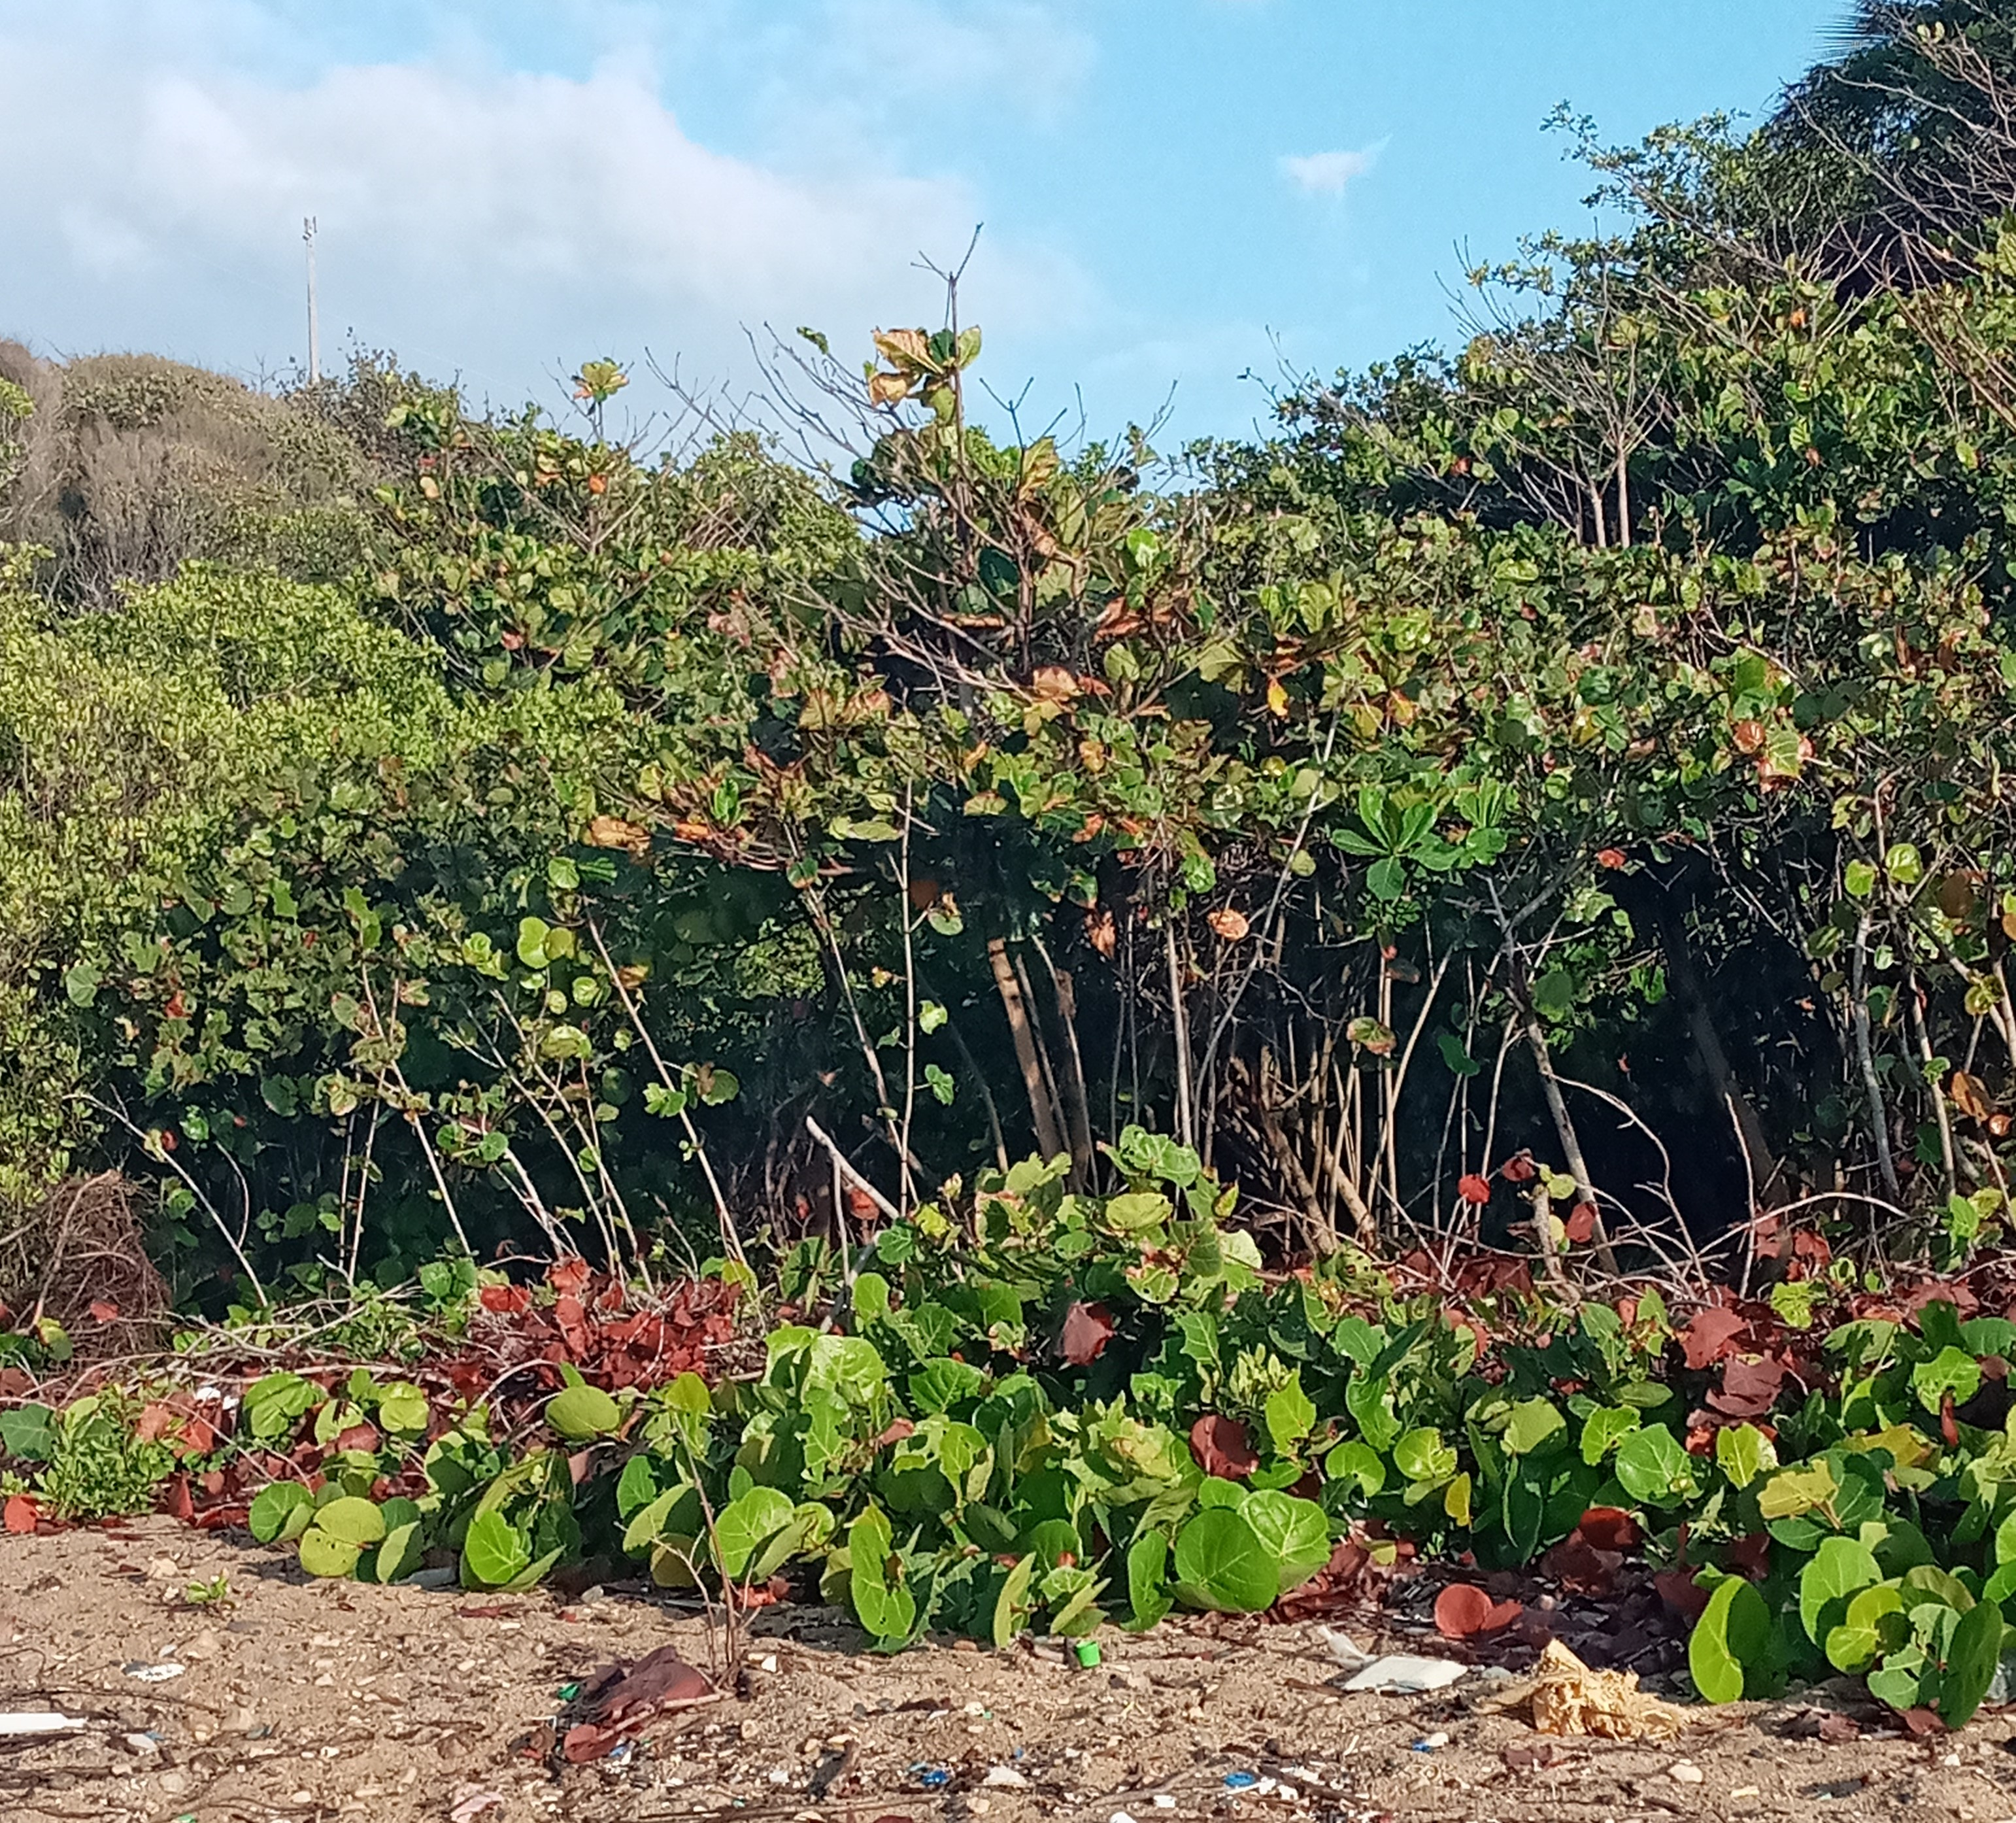
\includegraphics[height=3.12500in]{Cocoloba_uvifera.jpg}
\caption{Vegetación dunas de playa\label{cocoloba}}
\end{figure}

\begin{figure}
\centering
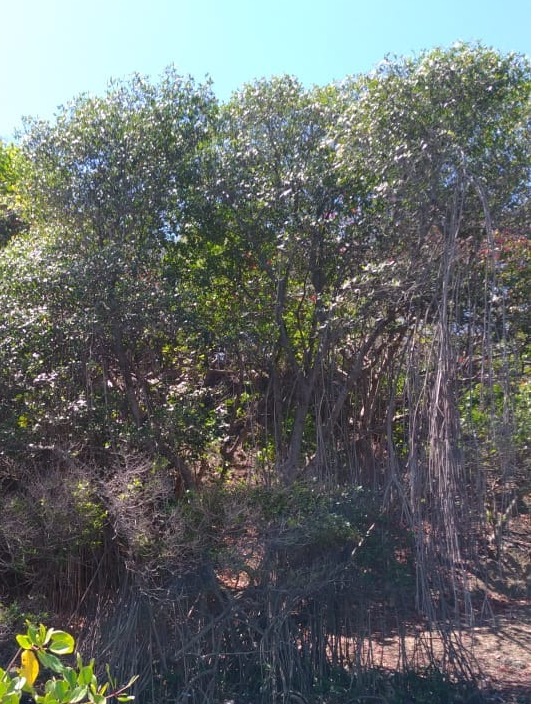
\includegraphics[height=3.64583in]{mangle_rojo.png}
\caption{Manglar\label{manglerojo}}
\end{figure}

\begin{figure}
\centering
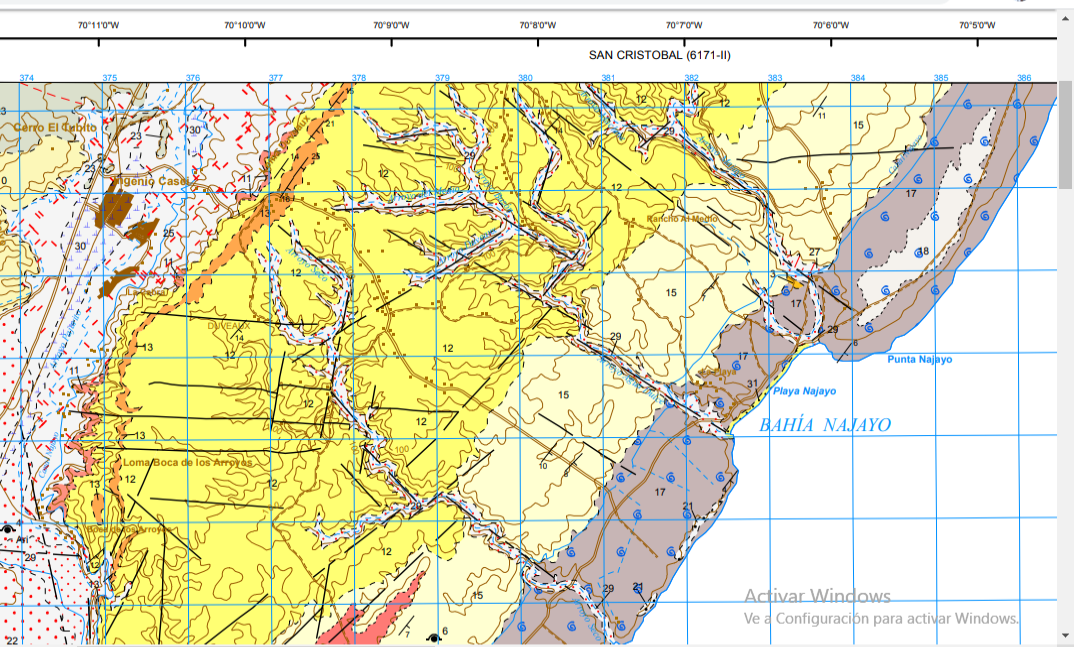
\includegraphics{mapa_bahia_najayo.png}
\caption{Mapa geológico escala 1:50,000 (hoja Nizao)\label{mapageo50k}}
\end{figure}

\ldots

\section{Metodología}\label{metodologuxeda}

Para cumplir los objetivos se emplearon varias técnicas, entre las que
se incluyen fotogrametría, navegación por satélite, teledetección,
sistemas de información geográfica y estadística.

Los cambios en el trazado de la línea de costa se analizaron utilizando
imágenes satelitales de Landsat 8 adquiridas entre los años 2013 y 2019.
De cada escena se extrajo la línea de costa empleando el algoritmo
CoastSat, el cual es un conjunto de herramientas escritas en Python, que
permite al usuario obtener series de tiempo de la posición de la costa
(Elsevier, n.d.).

Al delimitar las líneas de la costa, posteriormente se utilizó la
aplicación (QGIS y otros, n.d.) donde se seleccionaron los trazados de
mayor precisión teniendo como referencia la línea más antigua (2013),
dentro de dicho entorno gráfico se digitalizaron 25 transectos
perpendiculares a la dirección general del diseño. Finalmente, tanto los
transectos como las líneas fueron analizadas en R utilizando el script
RCoastSat (Batlle, 2020; R Core Team, 2020), el cual produjo resultados
gráficos que facilitaron la interpretación.

Asimismo, se colectaron muestras de sedimentos en siete puntos de
muestreos, los cuáles fueron seleccionados en base a tres áreas con
respecto al mar (canal,berma y duna de playa) e identificadas con un
código de lugar (AV2021,AV2529,AV2020,AV2010,AV8920,AV2510,AV2907)(ver
figura \ref{muestras}). Dichas muestras fueron depositadas en bolsas
Whirl Pak de 23 cm L x 11.5 cm W, con 0.064 mm de grosor y 532 ml de
capacidad. También, se tomaron las coordenadas de cada punto con el
receptor GPS convencional del telefono personal y se midieron los
clastos (en milímitros) presentes con una regla en dos ejes (largo y
ancho). Estos datos fueron rellenados en un formulario electrónico para
cada muestra, utilizando la aplicación ODK Collection (Singh, 2013)
descargada en el teléfono. Además, se extrajo por medio de un martillo
un fragmento del \emph{beachrock} (ver figura \ref{clasto}) al cuál se
le aplicó ácido clorhídrico para determinar si contenía carbonato.
Finalmente, para tener datos recientes del perfil de la playa, se
realizó un vuelo de dron y se tomaron fotografias de la zona.

\ldots

\section{Resultados}\label{resultados}

Los resultados generados se agrupan en tres subconjuntos:compilación de
trazados en la líneas de costa, colecta de sedimentos y las formaciones
de rocas en el centro de la playa, además de la restitución fotométrica
para la obtención de información tridimensional.

\subsection{Cambio de líneas de
costa}\label{cambio-de-luxedneas-de-costa}

Los trazados de las líneas de costa y los 25 transectos permitieron
reconstruir una serie de temporal de la dinámica del litoral de Najayo
(ver figura \ref{transecto}). Estos transectos muestran un esquema del
cambio de la costa por trimestre de cada año (ver figura \ref{cambio}).
También se identificaron los sectores de la playa más susceptibles al
cambio y las épocas del año de mayor actividad (ver tabla de
resultados\ref{resultados}). De manera global, los cambios más
prominentes ocurrieron en el tercer cuatrimestre (septiembre-diciembre)
de cada año, en los que comúnmente, predominó la progradación en casi
todos los años. Por el contrario, durante los meses de junio a agosto,
se registró una dinámica predominante de retrogradación.

Con respecto a, el perfil de playa las pendientes generadas de manera
dimensional presentaron la inclinación y a escala diferentes de varios
transectos a medida en que avanza al extremo occidental de la misma.
Ejemplos, de estos son los puntos desde el 11 hasta el 20 qué es donde
la playa inició a obtener alturas relevantes. De manera que, el 13
alcanzó un declive de poco más de 0.2 m y medio. Mientras que, en el 18
los cambios mostraron valores diferente, pero ninguno menores a los 0.10
m y medio (ver figura \ref{dimensional}). De igual manera, al emplearle
una misma escala existió una leve variación donde el 12 y 13 reflejaron
cambios superiores a los 0.2 m (ver figura \ref{escala}). Por otra
parte, en los puntos 32 y 33 la pendiente alcanzó un nivel superior con
escalas diferentes y su forma es más pronunciada (ver figura
\ref{pendiente}). En tanto que, con una misma el 33 y 37 proyectaron una
variación ligera de poco menos de 1 m (ver figura \ref{consistente}). En
relación con, el índice de concavidad la forma de la pendiente concuerda
en todos los transectos desde el 11 hasta el 40, aunque en algunos casos
uno menor que otro, excepto el 20 y 35 que presentó una forma diferente
(ver figura \ref{concavidad} y (ver figura \ref{indice}.

\subsubsection{Análisis
granulométrico}\label{anuxe1lisis-granulomuxe9trico}

El tamaño de los sedimentos presentó variaciones en cada punto de
muestreo (ver tabla\ref{estadistico}), donde se resumen los estadístico
y tamaños de muestra en cada una de las localidades de colecta (ver
tabla\ref{grafico} y tabla\ref{lugar}). La playa de los Pescadores
registró los valores extremos, tanto de ancho como de largo de los
clastos. Por otra parte, en las muestras de Carlos Pinto, los clastos
fueron más largo en promedio que en la otra playa.

En los diagramas de caja y en los histogramas se observa que las
muestras presentan sesgos hacia la derecha o positivo en ambas playas
(ver gráfico largo\ref{largo} y ancho\ref{ancho}). Adicionalmente, se
identificó la distribución por cuartiles de las mediciones según playa
(ver gráfico playa\ref{playa}). En la playa los Pescadores el 25\% más
pequeño de los clastos alcanzó 10 mm de largo y 7 mm de ancho, la
mediana (el valor que mide la muestra en dos partes iguales) fue de 13
mm y 10 mm para el largo y el ancho respectivamente, mientras que el
tercer cuartil, es decir el 75\% más pequeño de los clastos medidos
tenía 15 mm o menos de largo y 12 mm de ancho. En tanto que, en Carlos
Pinto la mediana fue de 15 mm y 9 mm de largo y ancho respectivamente y
el primer cuartil de 13 mm de largo y 8 mm de largo de aproximación.

\paragraph{Rocas de playa}\label{rocas-de-playa}

Las rocas emergidas y submergidas en la playa de Carlos Pinto se ubican
en el centro de la costa. Las mismas no exhiben elevadas altura, excepto
las que se encuentran cerca a los pequeños acantilados. Estas se
extienden desde la superficie terrestre hacia el mar, principalmente
desde el desagüe de dos drenaje de agua continental.

\begin{figure}
\centering
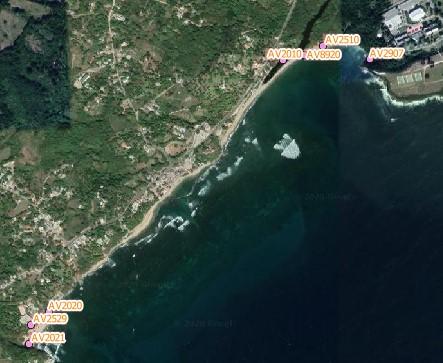
\includegraphics[height=2.60417in]{areas_muestras_colectadas.jpg}
\caption{Áreas de muestras colectadas\label{muestras}}
\end{figure}

\begin{figure}
\centering
\includegraphics[height=2.60417in]{Clasto_beachrock.jpg}
\caption{Composición de la roca de playa\label{clasto}}
\end{figure}

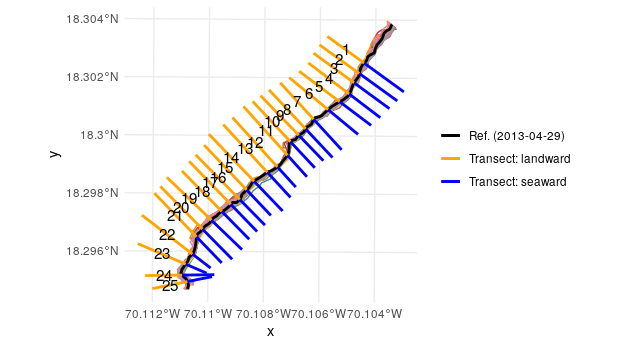
\includegraphics[height=3.64583in]{transect_linea_R.png} La línea de
color negro representa el trazado de referencia, el cual fue extraído de
la imágen satélital del año 2013. Los transectos de color amarillo
representan la superficie terrestre en tanto que los de azul el mar.

\begin{figure}
\centering
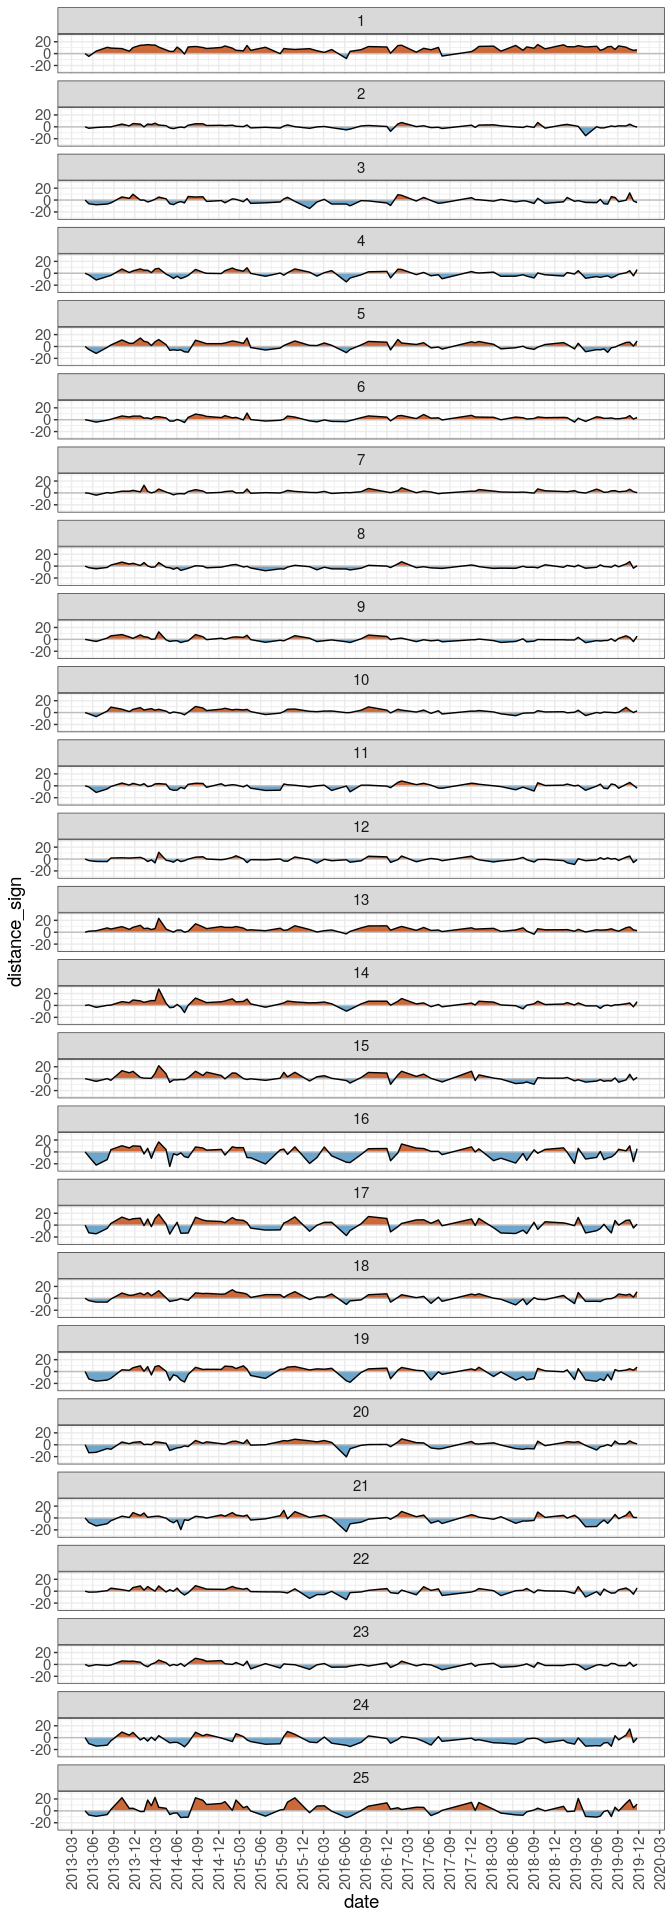
\includegraphics[height=3.12500in]{cambio_playa_Najayo.png}
\caption{Transectos sobre las líneas costera de
playa\_Najayo\label{cambio}}
\end{figure}

\begin{figure}
\centering
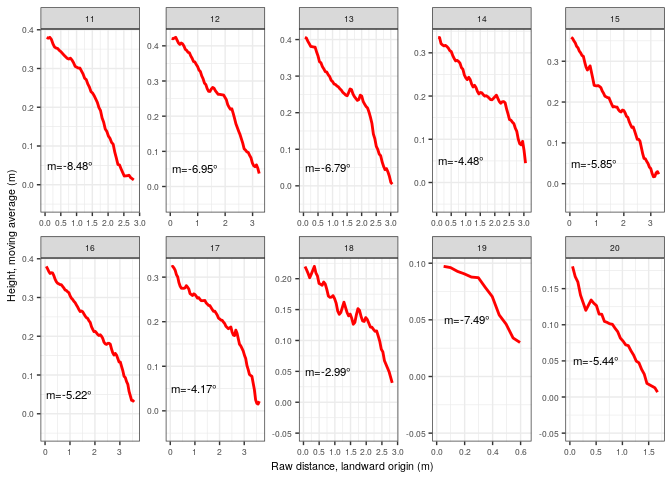
\includegraphics[height=2.60417in]{dimension_real.png}
\caption{Perfil dimensional de la playa\label{dimensional}}
\end{figure}

\begin{figure}
\centering
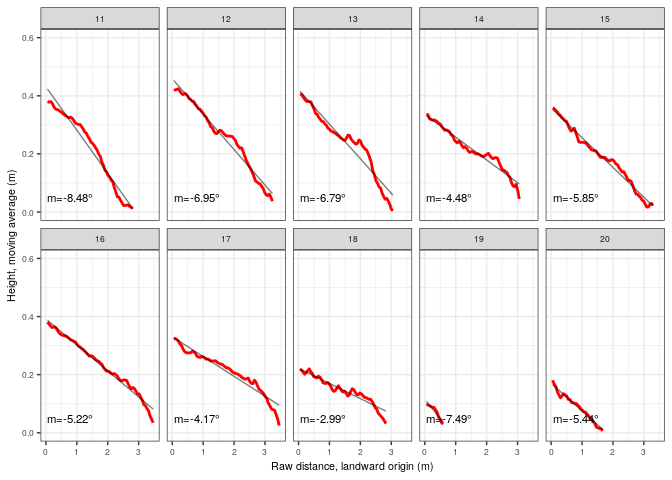
\includegraphics[height=2.60417in]{escala_diferente_consistente.png}
\caption{Perfil de playa con una misma escala\label{escala}}
\end{figure}

\begin{figure}
\centering
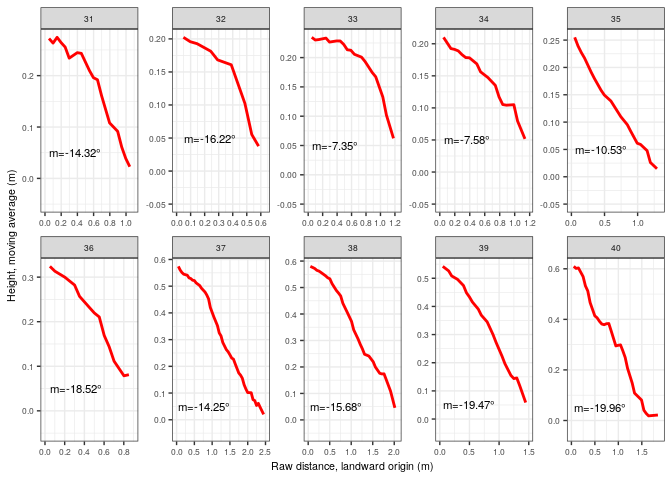
\includegraphics[height=2.60417in]{dimension_31-40.png}
\caption{Perfil de playa con varias escalas\label{pendiente}}
\end{figure}

\begin{figure}
\centering
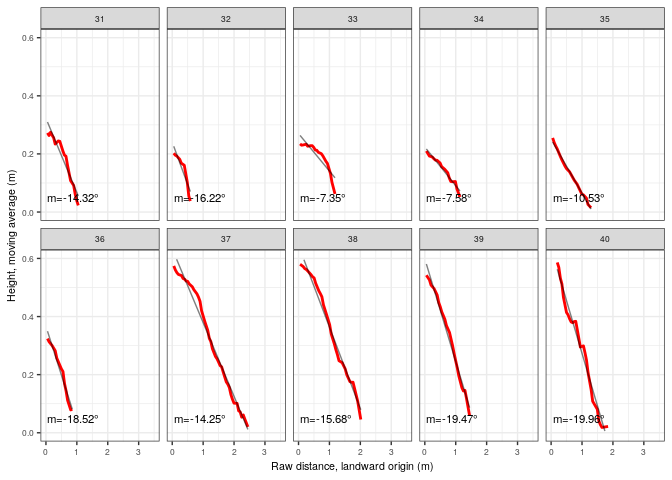
\includegraphics[height=2.60417in]{escala_diferente_consistente_31-40.png}
\caption{Perfil de playa con una misma escala\label{consistente}}
\end{figure}

\begin{figure}
\centering
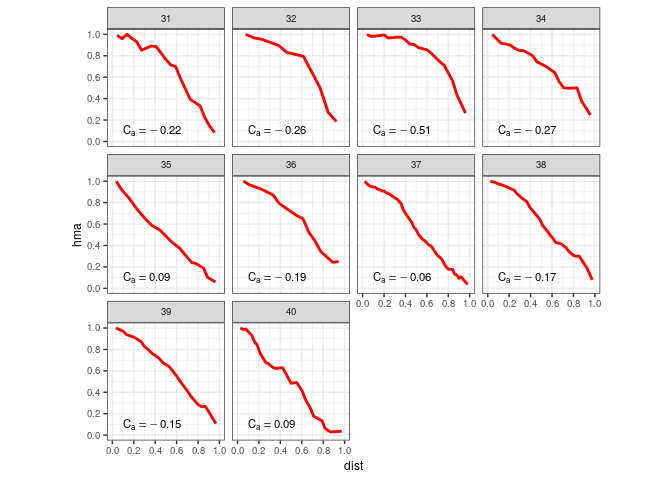
\includegraphics[height=2.60417in]{indice_concavidad.png}
\caption{Perfil con índice de concavidad\label{concavidad}}
\end{figure}

\begin{figure}
\centering
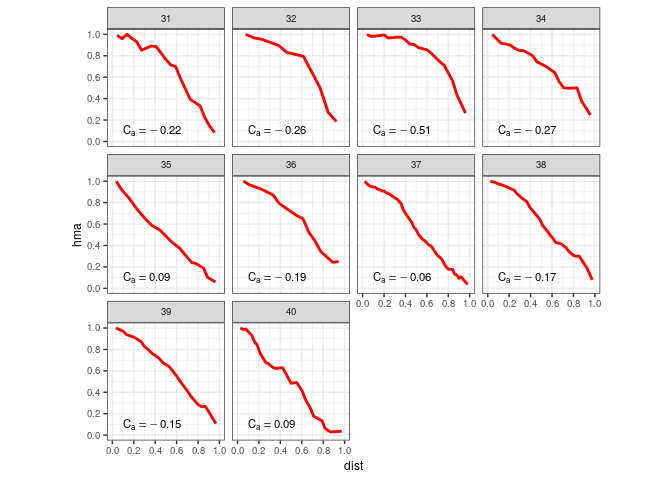
\includegraphics[height=2.60417in]{indice_concavidad_31-40.png}
\caption{Perfil con índice de concavidad\label{indice}}
\end{figure}

\begin{figure}
\centering
\includegraphics[height=2.60417in]{Beachrock.jpg}
\caption{Afloramiento de rocas playa\_Najayo\label{beachrock}}
\end{figure}

\begin{figure}
\centering
\includegraphics[height=2.60417in]{Arroyo_Aguadulce.jpg}
\caption{Desembocadura arroyo Agua Dulce
Playa\_Carlos\_Pinto\label{arroyo_aguadulce}}
\end{figure}

\begin{figure}
\centering
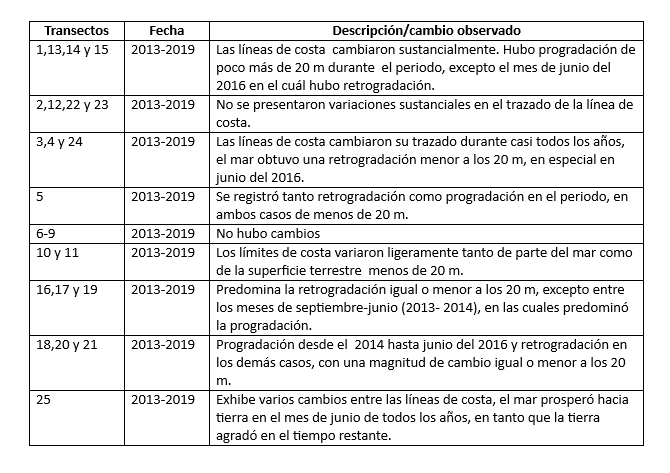
\includegraphics[height=2.60417in]{resultados_cambio_lineas.png}
\caption{Resultados cambios en la líneas de costa\label{resultados}}
\end{figure}

\begin{figure}
\centering
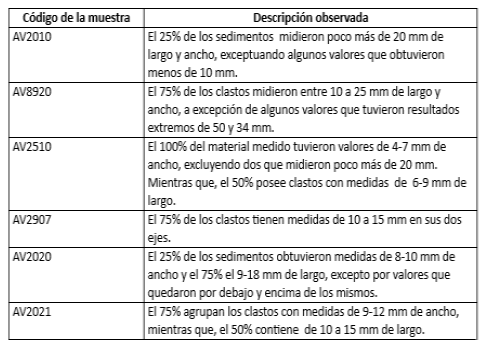
\includegraphics[height=2.60417in]{resultados_estadisticos.png}
\caption{Análisis estadísticos de las muestras\label{estadistico}}
\end{figure}

\begin{figure}
\centering
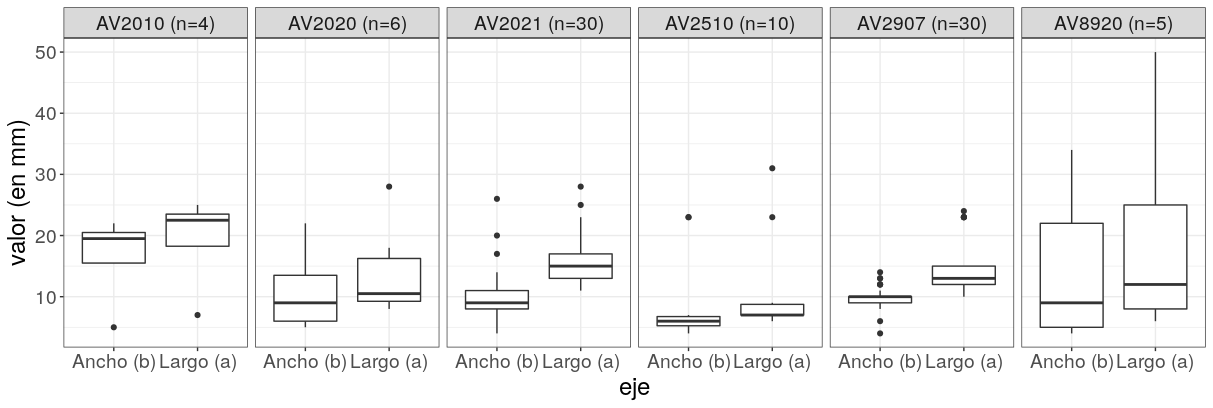
\includegraphics{muestra_graf.png}
\caption{Diagrama de las muestras\label{grafico}}
\end{figure}

\begin{figure}
\centering
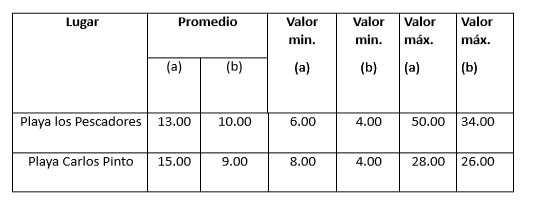
\includegraphics{tabla_lugar.png}
\caption{Resultados estadísticos de las playas \label{lugar}}
\end{figure}

\begin{figure}
\centering
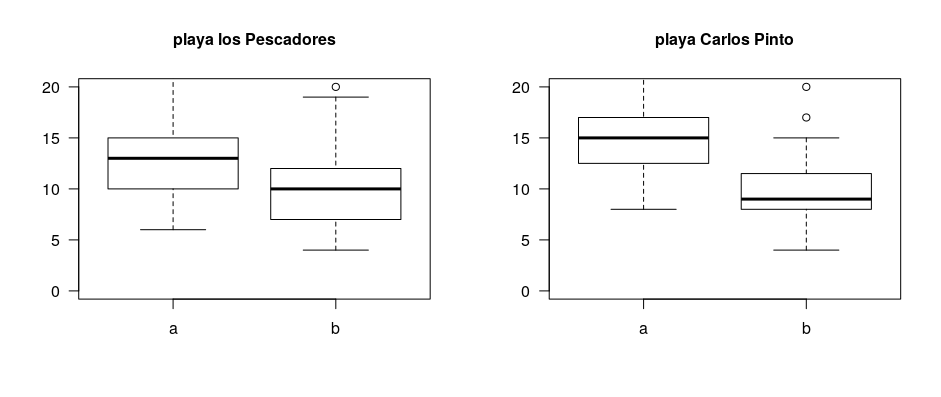
\includegraphics{diagrama.png}
\caption{Gráfico de las muestras por área de estudio\label{grafplaya}}
\end{figure}

\begin{figure}
\centering
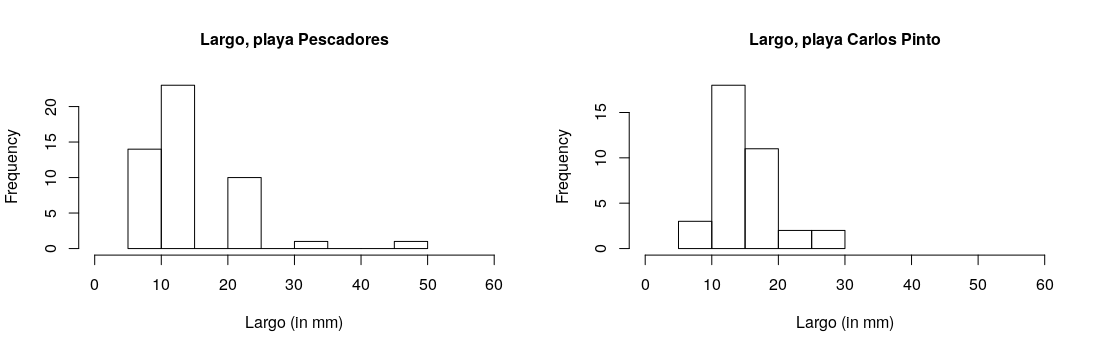
\includegraphics{largo_hist.png}
\caption{Histograma de largo\label{largo}}
\end{figure}

\begin{figure}
\centering
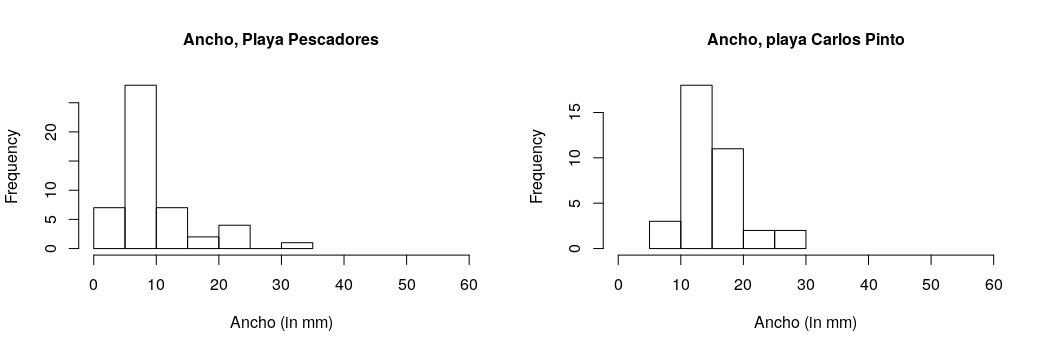
\includegraphics{ancho_hist.png}
\caption{Histograma de ancho\label{ancho}}
\end{figure}

\ldots

\section{Discusión}\label{discusiuxf3n}

\subsection{Cambio en líneas de
costa}\label{cambio-en-luxedneas-de-costa}

Los cambios presentados en las líneas de costa y en épocas específicas,
provablemente sean productos en su momento del incremento en el nivel
del mar, a concecuencia de fenomenos atmosféricos (tormentas/huracanes).
De cuerdo con Domínguez, Gracia, \& Anfuso (2004), estos fenomenos
originan fuertes oleajes que modifican la playa en un periodo
determinado. Esto, haciendo referencia de que el trimestre
junio-septiembre de todos los años presentó variaciones en todos los
trazados, donde predominó la retrogradación. Exceptuando, la temporada
del 2016 que fue la que más cambio mostró superando los 20 m de
distancia, posiblemetente por el paso del huracán Mathews (catégoria
tres) el cuál se encontraba al suroeste de Santo Domingo de acuerdo a un
periodico de circulación nacional. Además, esos cambios fueron
relevantes en áreas específicas de la costa, por ejemplo, la Playa de
Carlos Pinto fue más propensa a mostrar alteraciones, quizas por la
dirección de los vientos y la corriente marina que van erosionando la
morfología del litoral. Según Domínguez et al. (2004), el viento y el
oleaje provocan concentración o disipan energía, los cuales determinarán
mayor o menor erosión o incluso sedimentación.

Por otra parte, la playa presentó un perfil cóncavo donde la pendiente
fue tomando altura a medida que se acercaba a la desembocadora del
arroyo Agua Dulce al extremo occidental. Esta características se le
puede atribuir a la erosión a causa del oleaje, el viento y la corriente
marina que de acuerdo con (Lorenzo, Alonso, \& Pagés, 2003), la deriva
litoral es la causante de este proceso y el mismo puede ser diferente
durante cada estación del año. También, por la carga de sedimento de
parte del arroyo, razón de que en esta zona la inclinación fue mayor.

\subsubsection{Análisis
granulométrico}\label{anuxe1lisis-granulomuxe9trico-1}

Las variaciones en los tamaños presentados de los depósitos de
sedimentos en la playa de Najayo provablemente sean inusuales. En el
caso de, la playa los Pescadores que posee los valores más extremos en
cuanto a largo y ancho, potencialmente se deba a la dinámica de
transporte de sedimento existente en la zona. Puesto que, el arroyo
Rolón mantiene su recorrido (de forma lenta) hacia el mar, sedimentando
la costa constantemente. En relación con, Carlos Pinto que obtuvo el
promedio más largo y ancho, el cuál se le pude atribuir al flujo de
material arrastrado por el arroyo Agua Dulce en su tiempo de caudal. De
acuerdo con Kokot (2004) el cuál plantea que las aguas continentales son
las principales fuente de aportación de sedimentos en la costa y los
mismos son originarios de periodos donde las condiciones climáticas eran
diferentes de las actuales. De ahí, las diferencias en los clastos,
además de tener encuenta el tamaño de la cuenca, que en el caso de Agua
Dulce es de menor dimensión que el Rolón. Por otra parte, se deba a
fenómenos naturales, puesto que, en ese tiempo el mar excede su límite y
lanza escombros en toda la ensenada.

\paragraph{\texorpdfstring{\emph{Beachrock}}{Beachrock}}\label{beachrock}

Las rocas de playa se encuentran ubicadas en el espacio por el cuál
cañadas vierten sus aguas al mar, extendiéndose hacia el centro de la
costa. Posiblemente, éstas se formaron por la compactación de la arena
con el carbonato de calcio, es factible que en éste proceso de
fosilización el agua continental circulara de manera superficial por
rocas calizas arrecifales. El \emph{beachrock} presenta rocas alteradas
de basaltos, fósiles y tonalidas las cuales provablemente hallan emanado
del continente y eventualmente llevadas hasta ese lugar por la deriva
continental, por la cañada que desemboca en el mar o por un arroyo/río
que tal vez hoy ya no transita en el lugar.

\section{Agradecimientos}\label{agradecimientos}

Expresamos nuestro agradecimiento a la Universidad Autónoma de Santo
Domingo (UASD), en especial a la escuela de geografía por su deseo de
formar profesionales capaces de desarrollar habilidades críticas
fomentada en la investigación. También, al profesor José Ramón Martínez
Batlle por facilitar todas las herramientas de obteción de datos, por su
siempre disposición, ayuda e insistir en la importancia de los estudios
de investigación científica para la generación de conocimiento y
desarrollo de los pueblos. Por último, a Carolaine Pérez Ureña por
unirse a este tema de investigación y así generar información sobre el
litoral a favor de la sección Playa Najayo la cuál es escasa.

\section{Información de soporte}\label{informaciuxf3n-de-soporte}

\ldots

\section{\texorpdfstring{\emph{Script}
reproducible}{Script reproducible}}\label{script-reproducible}

\subsection{Packages}\label{packages}

\begin{Shaded}
\begin{Highlighting}[]
\KeywordTok{library}\NormalTok{(tidyverse)}
\KeywordTok{library}\NormalTok{(purrr)}
\KeywordTok{library}\NormalTok{(sf)}
\KeywordTok{library}\NormalTok{(RColorBrewer)}
\end{Highlighting}
\end{Shaded}

\subsection{Read the functions}\label{read-the-functions}

\begin{Shaded}
\begin{Highlighting}[]
\NormalTok{basegeofispath <-}\StringTok{ 'https://raw.githubusercontent.com/geofis/RCoastSat/master/R/'}
\NormalTok{scripts <-}\StringTok{ }\KeywordTok{c}\NormalTok{(}\StringTok{'classify-transects.R'}\NormalTok{, }\StringTok{'extract-points-distances.R'}\NormalTok{,}
             \StringTok{'interpolate.R'}\NormalTok{, }\StringTok{'read-shorelines.R'}\NormalTok{, }\StringTok{'read-transects.R'}\NormalTok{)}
\KeywordTok{invisible}\NormalTok{(purrr}\OperatorTok{::}\KeywordTok{map}\NormalTok{(}\KeywordTok{paste0}\NormalTok{(basegeofispath, scripts), }\ControlFlowTok{function}\NormalTok{(x) devtools}\OperatorTok{::}\KeywordTok{source_url}\NormalTok{(x)))}
\end{Highlighting}
\end{Shaded}

\begin{verbatim}
## SHA-1 hash of file is c5f094a166aafc99756ca04c86ac436dba34b942
\end{verbatim}

\begin{verbatim}
## SHA-1 hash of file is 1625bf00e42b93784549e9c6c5599ae0aa813ed1
\end{verbatim}

\begin{verbatim}
## SHA-1 hash of file is 51da8bcb0f875d3cd9ca72fa0a2e6a4435cacd06
\end{verbatim}

\begin{verbatim}
## SHA-1 hash of file is 366345fab0081871b6aa75ff1cadcfe80768bde7
\end{verbatim}

\begin{verbatim}
## SHA-1 hash of file is 2a2e9fca546c36437aed8394e6bc93cbad4775c8
\end{verbatim}

\subsection{Import/plot transects and
shorelines}\label{importplot-transects-and-shorelines}

\begin{Shaded}
\begin{Highlighting}[]
\NormalTok{shl <-}\StringTok{ }\KeywordTok{rshl}\NormalTok{(}\StringTok{'data/najayo-l8-shorelines.geojson'}\NormalTok{) }\OperatorTok\StringTok{ }\KeywordTok{mutate}\NormalTok{(}
  \DataTypeTok{date=}\KeywordTok{as.Date}\NormalTok{(date)) }\CommentTok{#Shorelines}
\end{Highlighting}
\end{Shaded}

\begin{verbatim}
## Reading layer `najayo-l8-shorelines' from data source `/home/analaroja29/unidad-0-asignacion-99-mi-manuscrito-anavalera29/data/najayo-l8-shorelines.geojson' using driver `GeoJSON'
## Simple feature collection with 80 features and 4 fields
## geometry type:  LINESTRING
## dimension:      XY
## bbox:           xmin: 382567.5 ymin: 2023148 xmax: 383401.9 ymax: 2024170
## projected CRS:  WGS 84 / UTM zone 19N
\end{verbatim}

\begin{Shaded}
\begin{Highlighting}[]
\NormalTok{refl <-}\StringTok{ }\NormalTok{shl }\OperatorTok\StringTok{ }\KeywordTok{filter}\NormalTok{(date}\OperatorTok{==}\KeywordTok{min}\NormalTok{(date}
\NormalTok{                                 )) }\CommentTok{#Reference shoreline}
\NormalTok{rawtrans <-}\StringTok{ }\KeywordTok{rtrans}\NormalTok{(}\StringTok{'transectos_lineacosta.geojson'}\NormalTok{) }\CommentTok{#Raw transects}
\end{Highlighting}
\end{Shaded}

\begin{verbatim}
## Reading layer `transectos_lineacosta' from data source `/home/analaroja29/unidad-0-asignacion-99-mi-manuscrito-anavalera29/transectos_lineacosta.geojson' using driver `GeoJSON'
## Simple feature collection with 25 features and 0 fields
## geometry type:  LINESTRING
## dimension:      XY
## bbox:           xmin: 382416.4 ymin: 2023149 xmax: 383430.4 ymax: 2024110
## projected CRS:  WGS 84 / UTM zone 19N
\end{verbatim}

\begin{Shaded}
\begin{Highlighting}[]
\NormalTok{trans <-}\StringTok{ }\KeywordTok{transclas}\NormalTok{(}\DataTypeTok{tr =}\NormalTok{ rawtrans, }\DataTypeTok{rl =}\NormalTok{ refl}
\NormalTok{                   ) }\CommentTok{#Transects classified by seaward/landward sections}
\end{Highlighting}
\end{Shaded}

\begin{verbatim}
## Warning: attribute variables are assumed to be spatially constant
## throughout all geometries

## Warning: attribute variables are assumed to be spatially constant
## throughout all geometries
\end{verbatim}

\begin{verbatim}
## Warning in st_cast.sf(tmultiline, "LINESTRING"): repeating attributes for
## all sub-geometries for which they may not be constant
\end{verbatim}

\begin{Shaded}
\begin{Highlighting}[]
\NormalTok{cols <-}\StringTok{ }\KeywordTok{colorRampPalette}\NormalTok{(}\KeywordTok{brewer.pal}\NormalTok{(}\DecValTok{9}\NormalTok{,}\StringTok{'Set1'}\NormalTok{))(}\KeywordTok{nrow}\NormalTok{(shl))}
\KeywordTok{ggplot}\NormalTok{() }\OperatorTok{+}
\StringTok{  }\KeywordTok{geom_sf}\NormalTok{(}\DataTypeTok{data =}\NormalTok{ shl }\OperatorTok\StringTok{ }\KeywordTok{mutate}\NormalTok{(}\DataTypeTok{date =} \KeywordTok{factor}\NormalTok{(date)), }
          \DataTypeTok{color =}\NormalTok{ cols) }\OperatorTok{+}
\StringTok{  }\KeywordTok{geom_sf}\NormalTok{(}
    \DataTypeTok{data =}\NormalTok{ refl }\OperatorTok\StringTok{ }\KeywordTok{mutate}\NormalTok{(}\DataTypeTok{linetype =} \KeywordTok{paste0}\NormalTok{(}\StringTok{'Ref. ('}\NormalTok{, date, }\StringTok{')'}\NormalTok{)),}
    \KeywordTok{aes}\NormalTok{(}\DataTypeTok{color=}\NormalTok{linetype), }\DataTypeTok{lwd =} \DecValTok{1}\NormalTok{, }\DataTypeTok{show.legend =} 
      \StringTok{'line'}\NormalTok{) }\OperatorTok{+}
\StringTok{  }\KeywordTok{geom_sf}\NormalTok{(}
    \DataTypeTok{data =}\NormalTok{ trans }\OperatorTok\StringTok{ }\KeywordTok{mutate}\NormalTok{(}\DataTypeTok{sealand=}\KeywordTok{paste0}\NormalTok{(}\StringTok{'Transect: '}\NormalTok{, sealand)),}
    \KeywordTok{aes}\NormalTok{(}\DataTypeTok{color =}\NormalTok{ sealand), }\DataTypeTok{show.legend =} \StringTok{'line'}\NormalTok{, }\DataTypeTok{lwd =} \DecValTok{1}\NormalTok{) }\OperatorTok{+}
\StringTok{  }\KeywordTok{scale_color_manual}\NormalTok{(}
    \DataTypeTok{values =} \KeywordTok{c}\NormalTok{(}\StringTok{'black'}\NormalTok{, }\StringTok{'orange'}\NormalTok{, }\StringTok{'blue'}\NormalTok{)) }\OperatorTok{+}
\StringTok{  }\KeywordTok{geom_sf_text}\NormalTok{(}
    \DataTypeTok{data =}\NormalTok{ trans }\OperatorTok\StringTok{ }\KeywordTok{filter}\NormalTok{(sealand}\OperatorTok{==}\StringTok{'landward'}\NormalTok{) }\OperatorTok
\StringTok{      }\NormalTok{st_centroid, }\KeywordTok{aes}\NormalTok{(}\DataTypeTok{label =}\NormalTok{ transect),}
    \DataTypeTok{size =} \DecValTok{4}\NormalTok{) }\OperatorTok{+}
\StringTok{  }\KeywordTok{theme_minimal}\NormalTok{() }\OperatorTok{+}
\StringTok{  }\KeywordTok{theme}\NormalTok{(}\DataTypeTok{legend.title =} \KeywordTok{element_blank}\NormalTok{())}
\end{Highlighting}
\end{Shaded}

\begin{verbatim}
## Warning in st_centroid.sf(.): st_centroid assumes attributes are constant
## over geometries of x
\end{verbatim}

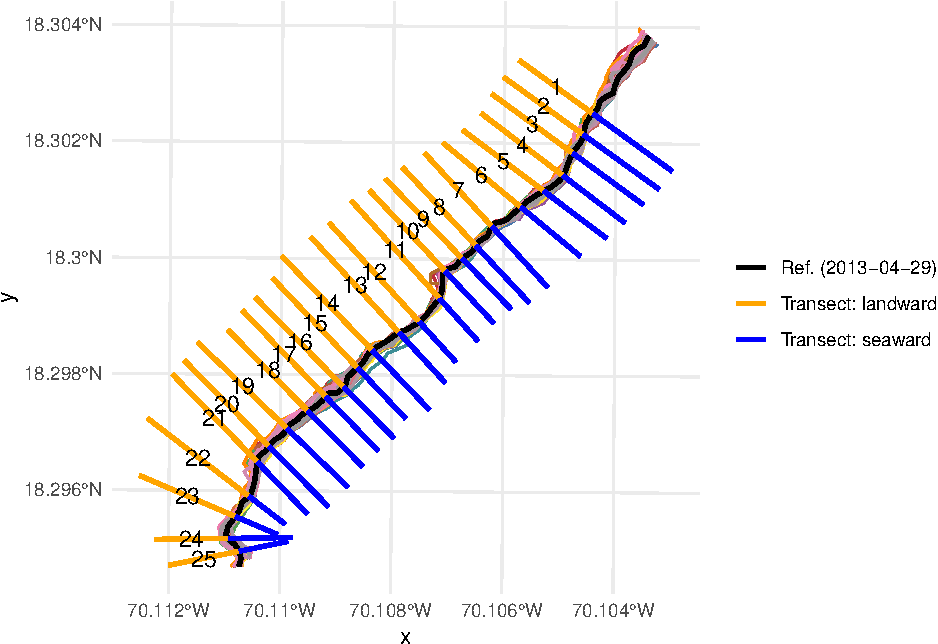
\includegraphics{manuscrito_files/figure-latex/unnamed-chunk-3-1.pdf}

\subsection{Extract points at interserctions and calculate
distances}\label{extract-points-at-interserctions-and-calculate-distances}

\begin{Shaded}
\begin{Highlighting}[]
\NormalTok{distl <-}\StringTok{ }\KeywordTok{pointdist}\NormalTok{(}\DataTypeTok{sh =}\NormalTok{ shl, }\DataTypeTok{re =}\NormalTok{ refl, }\DataTypeTok{tr =}\NormalTok{ trans, }\DataTypeTok{rtr =}\NormalTok{ rawtrans)}
\end{Highlighting}
\end{Shaded}

\begin{verbatim}
## Warning: attribute variables are assumed to be spatially constant
## throughout all geometries

## Warning: attribute variables are assumed to be spatially constant
## throughout all geometries
\end{verbatim}

\subsection{Time-series of shoreline change for each
transect}\label{time-series-of-shoreline-change-for-each-transect}

\begin{Shaded}
\begin{Highlighting}[]
\NormalTok{interdist <-}\StringTok{ }\KeywordTok{map}\NormalTok{(distl, interpolate) }\OperatorTok\StringTok{ }\NormalTok{plyr}\OperatorTok{::}\KeywordTok{ldply}\NormalTok{()}
\NormalTok{distances <-}\StringTok{ }\NormalTok{plyr}\OperatorTok{::}\KeywordTok{ldply}\NormalTok{(distl)}
\NormalTok{distances }\OperatorTok\StringTok{ }
\StringTok{  }\KeywordTok{ggplot}\NormalTok{() }\OperatorTok{+}\StringTok{ }\KeywordTok{theme_bw}\NormalTok{() }\OperatorTok{+}\StringTok{ }\KeywordTok{aes}\NormalTok{(}\DataTypeTok{x =}\NormalTok{ date, }\DataTypeTok{y =}\NormalTok{ distance_sign) }\OperatorTok{+}
\StringTok{  }\KeywordTok{geom_ribbon}\NormalTok{(}\DataTypeTok{data =}\NormalTok{ interdist, }\KeywordTok{aes}\NormalTok{(}\DataTypeTok{ymax =} \KeywordTok{pmax}\NormalTok{(distance_sign,}
                                                \DecValTok{0}\NormalTok{), }\DataTypeTok{ymin =} \DecValTok{0}\NormalTok{), }\DataTypeTok{fill =} \StringTok{"sienna3"}\NormalTok{) }\OperatorTok{+}
\StringTok{  }\KeywordTok{geom_ribbon}\NormalTok{(}\DataTypeTok{data =}\NormalTok{ interdist, }
              \KeywordTok{aes}\NormalTok{(}\DataTypeTok{ymin =} \KeywordTok{pmin}\NormalTok{(distance_sign, }\DecValTok{0}\NormalTok{), }\DataTypeTok{ymax =} \DecValTok{0}\NormalTok{), }\DataTypeTok{fill =} \StringTok{"skyblue3"}\NormalTok{) }\OperatorTok{+}
\StringTok{  }\KeywordTok{geom_hline}\NormalTok{(}\DataTypeTok{yintercept =} \DecValTok{0}\NormalTok{, }\DataTypeTok{color =} \StringTok{'grey'}\NormalTok{) }\OperatorTok{+}
\StringTok{  }\KeywordTok{geom_line}\NormalTok{(}\DataTypeTok{colour=}\StringTok{'black'}\NormalTok{, }\DataTypeTok{lwd =} \FloatTok{0.5}\NormalTok{) }\OperatorTok{+}
\StringTok{  }\KeywordTok{scale_x_date}\NormalTok{(}\DataTypeTok{labels =}\NormalTok{ scales}\OperatorTok{::}\KeywordTok{date_format}\NormalTok{(}\StringTok{"%Y-%m"}\NormalTok{), }
               \DataTypeTok{date_breaks =} \StringTok{'3 months'}\NormalTok{) }\OperatorTok{+}
\StringTok{  }\KeywordTok{scale_y_continuous}\NormalTok{(}\DataTypeTok{limits =} \KeywordTok{c}\NormalTok{(}\OperatorTok{-}\DecValTok{30}\NormalTok{, }\DecValTok{30}\NormalTok{)) }\OperatorTok{+}
\StringTok{  }\KeywordTok{theme}\NormalTok{(}\DataTypeTok{axis.text.x =} \KeywordTok{element_text}\NormalTok{(}\DataTypeTok{angle =} \DecValTok{90}\NormalTok{, }\DataTypeTok{vjust =} \FloatTok{0.5}
\NormalTok{                                   ), }\DataTypeTok{text =} \KeywordTok{element_text}\NormalTok{(}\DataTypeTok{size =} \DecValTok{14}\NormalTok{)) }\OperatorTok{+}
\StringTok{  }\KeywordTok{facet_wrap}\NormalTok{(}\OperatorTok{~}\NormalTok{transect, }\DataTypeTok{ncol =} \DecValTok{1}\NormalTok{)}
\end{Highlighting}
\end{Shaded}

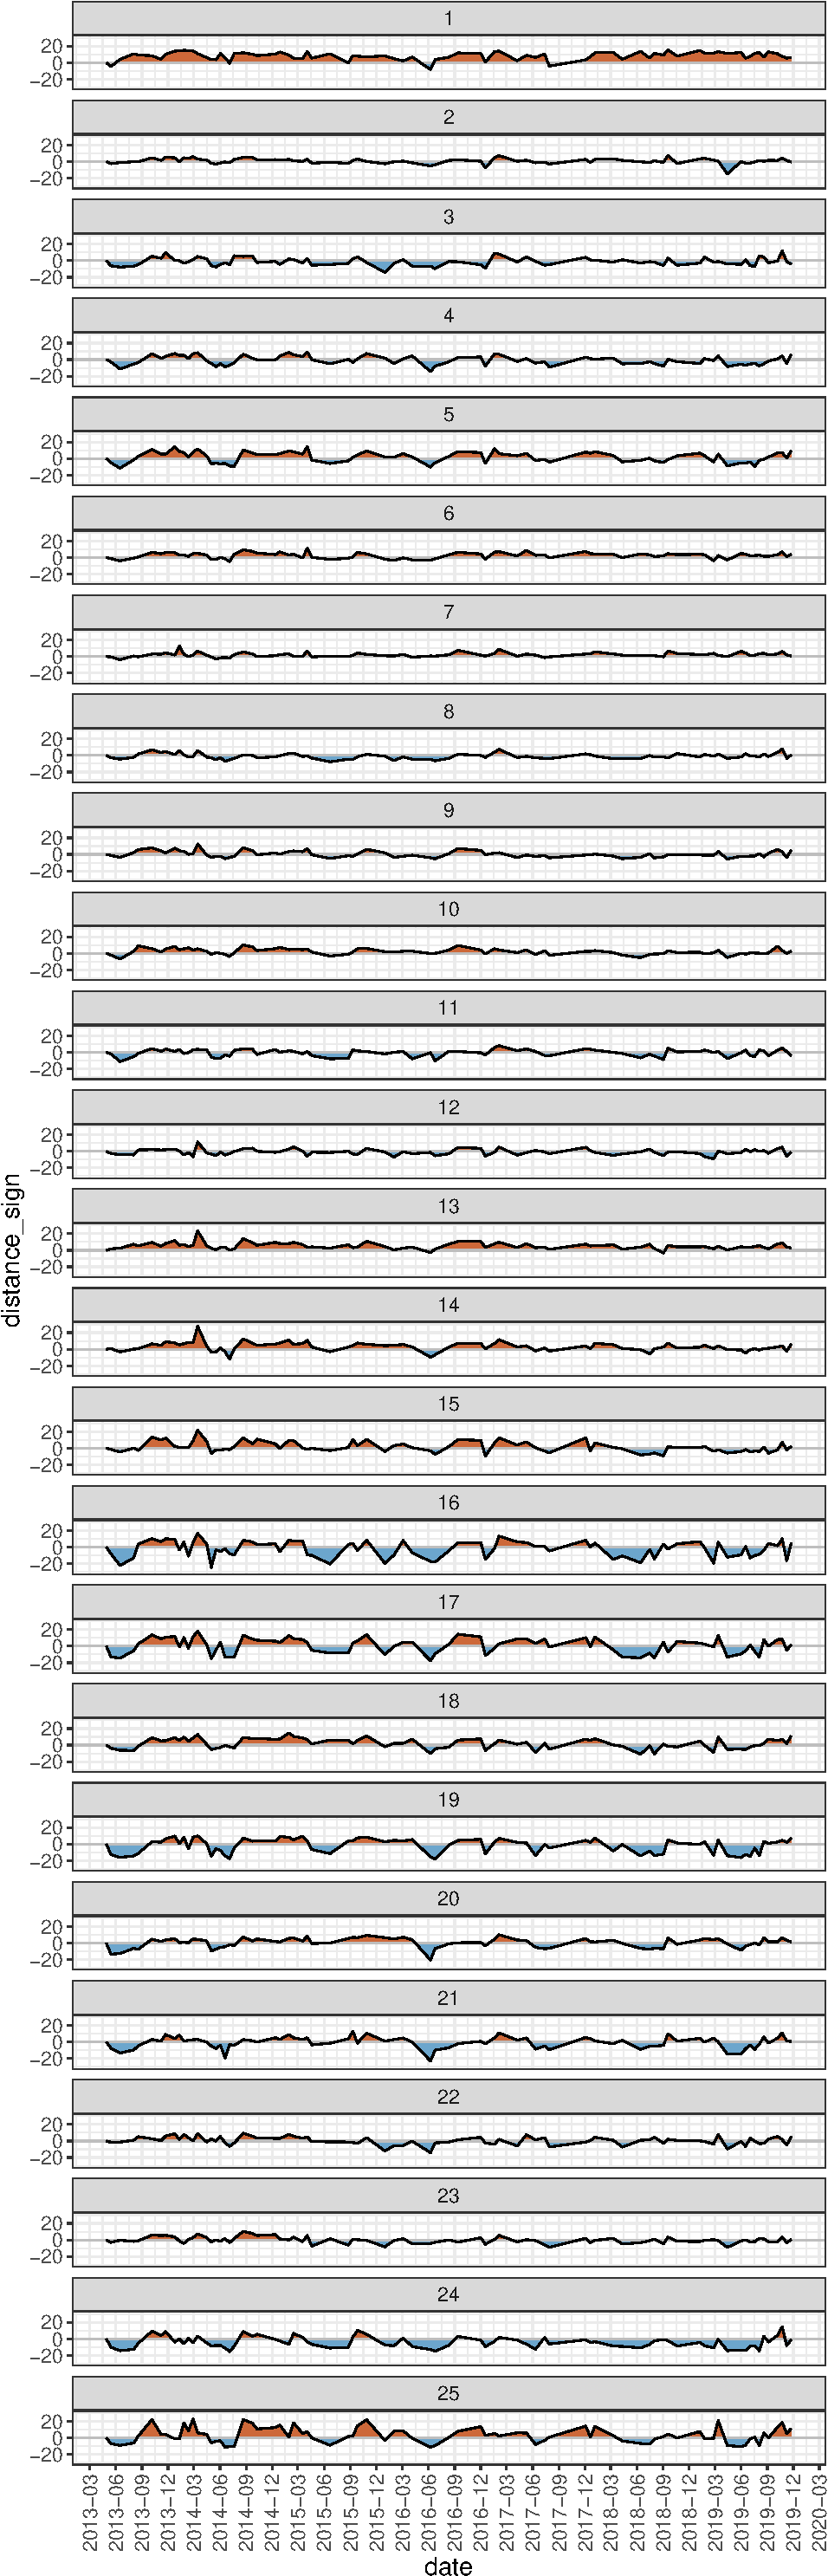
\includegraphics{manuscrito_files/figure-latex/unnamed-chunk-5-1.pdf}

\section{Análisis granulométrico}\label{anuxe1lisis-granulomuxe9trico-2}

\begin{Shaded}
\begin{Highlighting}[]
\KeywordTok{library}\NormalTok{(jsonlite)}
\end{Highlighting}
\end{Shaded}

\begin{verbatim}
## 
## Attaching package: 'jsonlite'
\end{verbatim}

\begin{verbatim}
## The following object is masked from 'package:purrr':
## 
##     flatten
\end{verbatim}

\begin{Shaded}
\begin{Highlighting}[]
\KeywordTok{library}\NormalTok{(tidyverse)}
\NormalTok{df <-}\StringTok{ }\NormalTok{jsonlite}\OperatorTok{::}\KeywordTok{fromJSON}\NormalTok{(}\StringTok{'Cantometría_3_results.json'}\NormalTok{, }\DataTypeTok{flatten =} \OtherTok{TRUE}\NormalTok{)}
\NormalTok{df  }\OperatorTok\StringTok{ }\KeywordTok{filter}\NormalTok{(}\OperatorTok{!}\NormalTok{codigomuestra }\OperatorTok\StringTok{ }\KeywordTok{c}\NormalTok{(}\StringTok{'C20190726M1'}\NormalTok{, }\StringTok{'C20191028M1'}
\NormalTok{                               )) }\OperatorTok\StringTok{ }\KeywordTok{unnest}\NormalTok{(clastos) }\OperatorTok
\StringTok{  }\KeywordTok{select}\NormalTok{(}\StringTok{`}\DataTypeTok{Codigo de lugar}\StringTok{`}\NormalTok{=codigomuestra, }\StringTok{`}\DataTypeTok{Largo (a)}\StringTok{`}\NormalTok{=a,}
         \StringTok{`}\DataTypeTok{Ancho (b)}\StringTok{`}\NormalTok{=b) }\OperatorTok
\StringTok{  }\KeywordTok{group_by}\NormalTok{(}\StringTok{`}\DataTypeTok{Codigo de lugar}\StringTok{`}\NormalTok{) }\OperatorTok
\StringTok{  }\KeywordTok{mutate}\NormalTok{(}\StringTok{'Codigo de lugar n'}\NormalTok{=}\KeywordTok{paste0}\NormalTok{(}\StringTok{`}\DataTypeTok{Codigo de lugar}\StringTok{`}\NormalTok{,}
                           \StringTok{' (n='}\NormalTok{, }\KeywordTok{length}\NormalTok{(}\StringTok{`}\DataTypeTok{Codigo de lugar}\StringTok{`}\NormalTok{),}\StringTok{')'}\NormalTok{)) }\OperatorTok
\StringTok{  }\KeywordTok{ungroup}\NormalTok{() }\OperatorTok\StringTok{ }\KeywordTok{select}\NormalTok{(}\OperatorTok{-}\StringTok{`}\DataTypeTok{Codigo de lugar}\StringTok{`}
\NormalTok{                       ) }\OperatorTok\StringTok{ }\KeywordTok{gather}\NormalTok{(eje,}
                    \StringTok{`}\DataTypeTok{valor (en mm)}\StringTok{`}\NormalTok{, }\OperatorTok{-}\StringTok{`}\DataTypeTok{Codigo de lugar n}\StringTok{`}\NormalTok{) }\OperatorTok
\StringTok{  }\KeywordTok{ggplot}\NormalTok{() }\OperatorTok{+}\StringTok{ }\KeywordTok{aes}\NormalTok{(}\DataTypeTok{x =}\NormalTok{ eje, }\DataTypeTok{y =} \StringTok{`}\DataTypeTok{valor (en mm)}\StringTok{`}\NormalTok{) }\OperatorTok{+}\StringTok{ }\KeywordTok{geom_boxplot}\NormalTok{() }\OperatorTok{+}
\StringTok{  }\KeywordTok{facet_grid}\NormalTok{(}\OperatorTok{~}\StringTok{`}\DataTypeTok{Codigo de lugar n}\StringTok{`}\NormalTok{) }\OperatorTok{+}\StringTok{ }\KeywordTok{theme_bw}\NormalTok{() }\OperatorTok{+}
\StringTok{  }\KeywordTok{theme}\NormalTok{(}\DataTypeTok{text =} \KeywordTok{element_text}\NormalTok{(}\DataTypeTok{size =} \DecValTok{18}\NormalTok{))}
\end{Highlighting}
\end{Shaded}

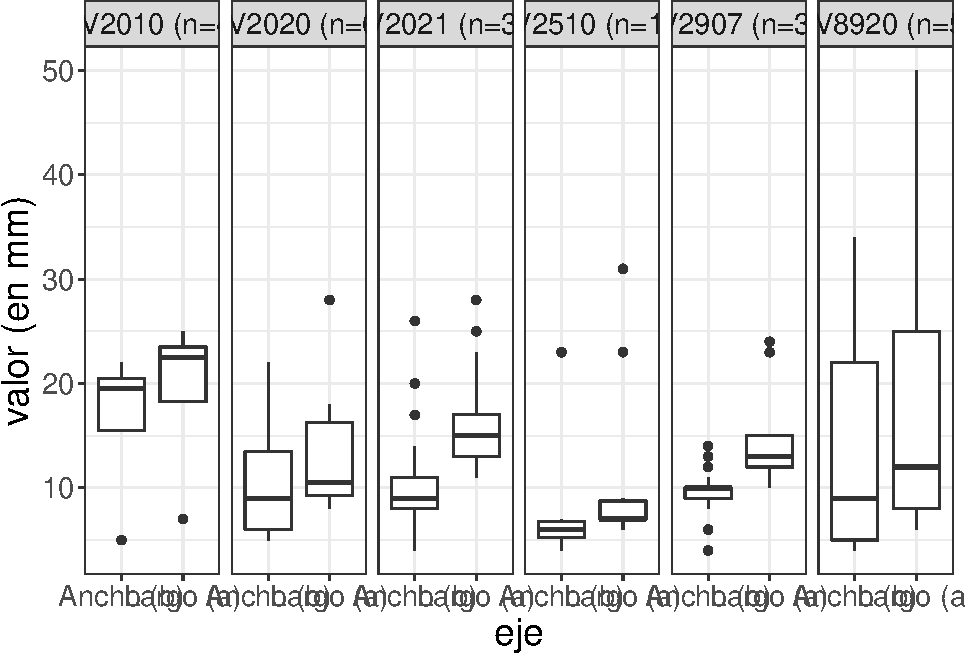
\includegraphics{manuscrito_files/figure-latex/unnamed-chunk-6-1.pdf}

\begin{Shaded}
\begin{Highlighting}[]
\NormalTok{df2 <-}\StringTok{ }\NormalTok{df }\OperatorTok\StringTok{ }\KeywordTok{filter}\NormalTok{(}\OperatorTok{!}\NormalTok{codigomuestra }\OperatorTok\StringTok{ }\KeywordTok{c}\NormalTok{(}\StringTok{'C20190726M1'}\NormalTok{,}
                      \StringTok{'C20191028M1'}\NormalTok{)) }\OperatorTok\StringTok{ }\KeywordTok{unnest}\NormalTok{(clastos)}

\NormalTok{playa_pescadores <-}\StringTok{ }\KeywordTok{droplevels}\NormalTok{(df2[df2}\OperatorTok{$}\NormalTok{codigomuestra }\OperatorTok\StringTok{ }\KeywordTok{c}\NormalTok{(}
  \StringTok{"AV2010"}\NormalTok{,}\StringTok{"AV8920"}\NormalTok{,}\StringTok{"AV2907"}\NormalTok{,}\StringTok{"AV2510"}\NormalTok{), }\KeywordTok{c}\NormalTok{(}\StringTok{"a"}\NormalTok{,}\StringTok{"b"}\NormalTok{)])}

\NormalTok{playa_carlos_pinto <-}\StringTok{ }\KeywordTok{droplevels}\NormalTok{(}
\NormalTok{  df2[df2}\OperatorTok{$}\NormalTok{codigomuestra }\OperatorTok\StringTok{ }\KeywordTok{c}\NormalTok{(}\StringTok{"AV2021"}\NormalTok{,}\StringTok{"AV2020"}\NormalTok{), }\KeywordTok{c}\NormalTok{(}\StringTok{"a"}\NormalTok{,}\StringTok{"b"}\NormalTok{)])}

\KeywordTok{par}\NormalTok{(}\DataTypeTok{mfrow=}\KeywordTok{c}\NormalTok{(}\DecValTok{1}\NormalTok{,}\DecValTok{2}\NormalTok{))}

\KeywordTok{boxplot}\NormalTok{(playa_pescadores, }\DataTypeTok{las =} \DecValTok{1}\NormalTok{, }\DataTypeTok{main =} \StringTok{'playa los Pescadores'}\NormalTok{, }
        \DataTypeTok{cex.main =} \DecValTok{1}\NormalTok{, }\DataTypeTok{ylim =} \KeywordTok{c}\NormalTok{(}\DecValTok{0}\NormalTok{,}\DecValTok{20}\NormalTok{))}

\KeywordTok{boxplot}\NormalTok{(playa_carlos_pinto, }\DataTypeTok{las =} \DecValTok{1}\NormalTok{, }\DataTypeTok{main =} \StringTok{'playa Carlos Pinto'}\NormalTok{,}
        \DataTypeTok{cex.main =} \DecValTok{1}\NormalTok{, }\DataTypeTok{ylim =} \KeywordTok{c}\NormalTok{(}\DecValTok{0}\NormalTok{,}\DecValTok{20}\NormalTok{))}
\end{Highlighting}
\end{Shaded}

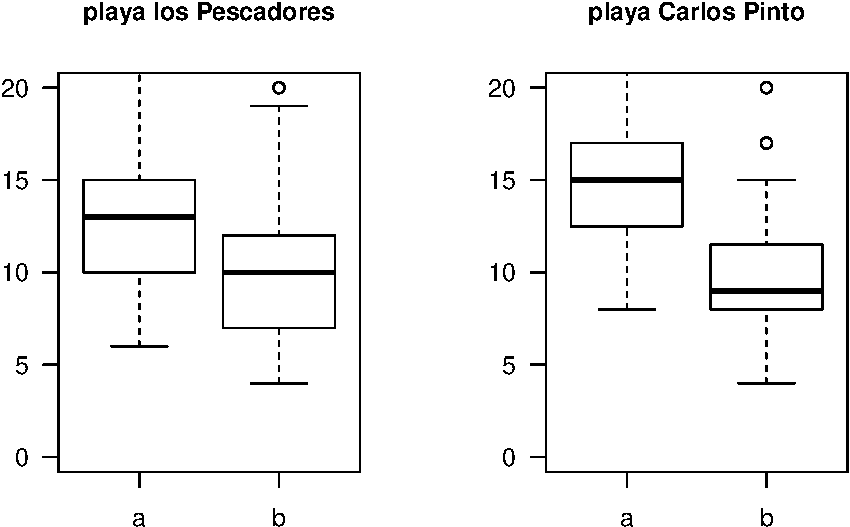
\includegraphics{manuscrito_files/figure-latex/unnamed-chunk-6-2.pdf}

\begin{Shaded}
\begin{Highlighting}[]
\KeywordTok{hist}\NormalTok{(playa_pescadores}\OperatorTok{$}\NormalTok{a, }\DataTypeTok{xlim =} \KeywordTok{c}\NormalTok{(}\DecValTok{0}\NormalTok{,}\DecValTok{200}\NormalTok{), }\DataTypeTok{main =} \StringTok{'Largo, playa Pescadores'}\NormalTok{,}
     \DataTypeTok{xlab =} \StringTok{'Largo (in mm)'}\NormalTok{, }\DataTypeTok{cex.main =} \DecValTok{1}\NormalTok{)}

\KeywordTok{hist}\NormalTok{(playa_carlos_pinto}\OperatorTok{$}\NormalTok{a, }\DataTypeTok{xlim =} \KeywordTok{c}\NormalTok{(}\DecValTok{0}\NormalTok{,}\DecValTok{200}\NormalTok{), }\DataTypeTok{main =} \StringTok{'Largo, playa Carlos Pinto'}\NormalTok{,}
     \DataTypeTok{xlab =} \StringTok{'Largo (in mm)'}\NormalTok{, }\DataTypeTok{cex.main =} \DecValTok{1}\NormalTok{)}
\end{Highlighting}
\end{Shaded}

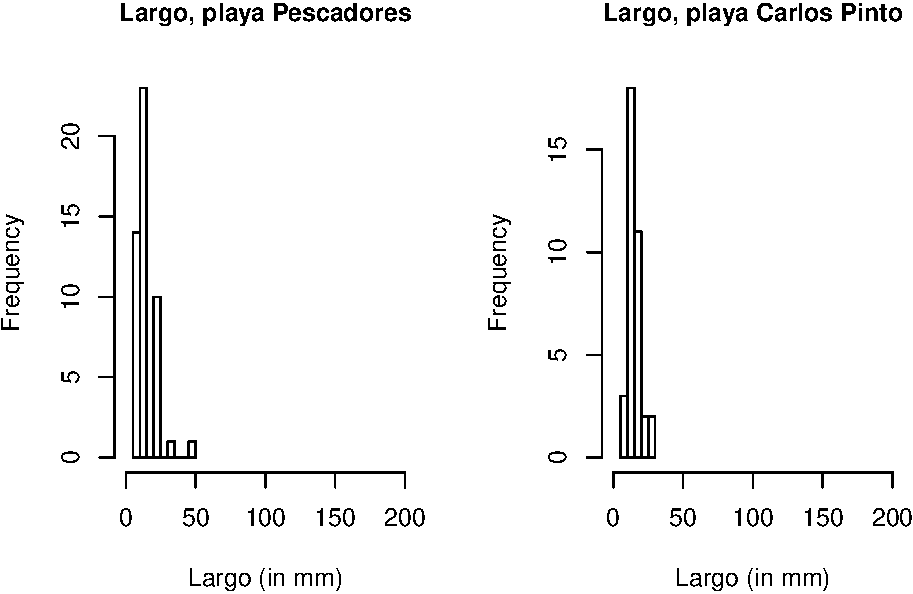
\includegraphics{manuscrito_files/figure-latex/unnamed-chunk-6-3.pdf}

\begin{Shaded}
\begin{Highlighting}[]
\KeywordTok{hist}\NormalTok{(playa_pescadores}\OperatorTok{$}\NormalTok{b, }\DataTypeTok{xlim =} \KeywordTok{c}\NormalTok{(}\DecValTok{0}\NormalTok{,}\DecValTok{200}\NormalTok{), }\DataTypeTok{main =} \StringTok{'Ancho, Playa pescadores'}\NormalTok{,}
     \DataTypeTok{xlab =} \StringTok{'Ancho (in mm)'}\NormalTok{, }\DataTypeTok{cex.main =} \DecValTok{1}\NormalTok{)}

\KeywordTok{hist}\NormalTok{(playa_carlos_pinto}\OperatorTok{$}\NormalTok{a, }\DataTypeTok{xlim =} \KeywordTok{c}\NormalTok{(}\DecValTok{0}\NormalTok{,}\DecValTok{200}\NormalTok{), }\DataTypeTok{main =} \StringTok{'Ancho, playa Carlos Pinto'}\NormalTok{,}
     \DataTypeTok{xlab =} \StringTok{'Ancho (in mm)'}\NormalTok{, }\DataTypeTok{cex.main =} \DecValTok{1}\NormalTok{)}
\end{Highlighting}
\end{Shaded}

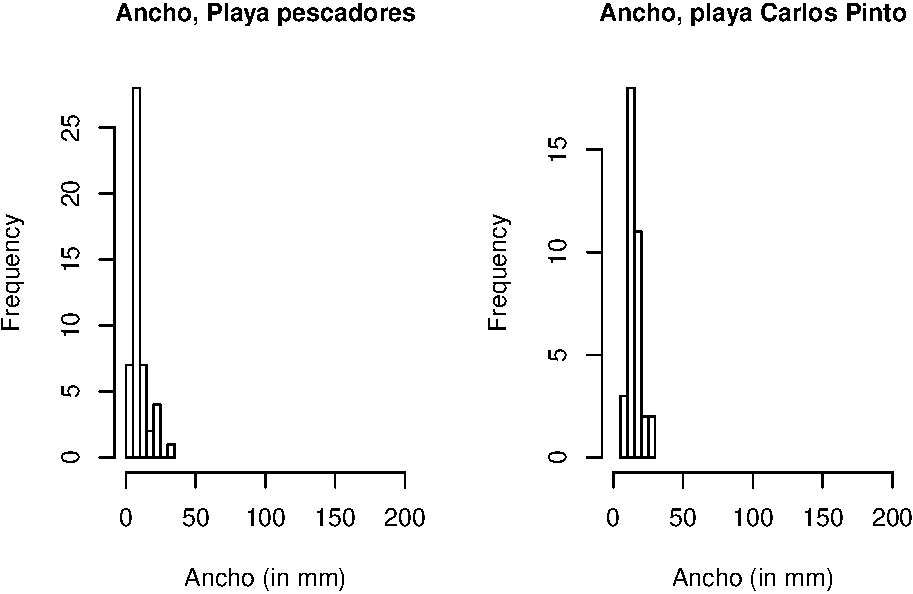
\includegraphics{manuscrito_files/figure-latex/unnamed-chunk-6-4.pdf}

\ldots

\section*{Referencias}\label{referencias}
\addcontentsline{toc}{section}{Referencias}

\hypertarget{refs}{}
\hypertarget{ref-abad2007mapageonizao}{}
Abad de los Santos, M. (. (2007--2010). \emph{Mapa Geológico de la
República Dominicana a escala 1:50.000 de la hoja n 6170-I (Nizao) y
Memoria correspondiente}. Santo Domingo: Proyecto 1B de Cartografía
Geotemática de la República Dominicana. Programa SYSMIN. Servicio
Geológico Nacional.

\hypertarget{ref-abreu1999impacto}{}
Abreu, L. (1999). Impacto del turismo en el litoral de dominicana.
\emph{Revista Geográfica}, 167--182.

\hypertarget{ref-aliotta2009origen}{}
Aliotta, S., Spagnuolo, J. O., \& Farinati, E. A. (2009). Origen de una
roca de playa en la región costera de bahía blanca, argentina.
\emph{Pesquisas Em Geociências}, \emph{36}(1), 107--116.

\hypertarget{ref-rcoastsat}{}
Batlle, J. R. M. (2020). \emph{RCoastSat}.
\href{\%0Ahttps://github.com/geofis/RCoastSat\%0A}{
https://github.com/geofis/RCoastSat
}.

\hypertarget{ref-camara1997republica}{}
Cámara Artigas, R. (1997). \emph{República dominicana: Dinámica del
medio físico en la región caribe (geografía física, sabanas y litoral)
aportación al conocimiento de la tropicalidad insular}.

\hypertarget{ref-cervantes2009evidencia}{}
Cervantes Guerra, Y. M., Almaguer Carmenates, Y., Orozco Melgar, G.,
Pierra Conde, A., \& Gursky, H. (2009). \emph{Evidencia documental de
los cambios geomorfológicos en cayo moa grande, moa, cuba.}

\hypertarget{ref-codignotto1997geomorfologia}{}
Codignotto, J. (1997). \emph{Geomorfología y dinámica costera}.

\hypertarget{ref-maparecursosminerales}{}
Diaz de Neira, A. (2007--2010). \emph{Mapa de recursos minerales de la
Repú Dominicana, escala 1:100,000}. Santo Domingo: Proyecto 1B de
Cartografía Geotemática de la República Dominicana. Programa SYSMIN.
Servicio Geológico Nacional.

\hypertarget{ref-dominguez2004tasas}{}
Domínguez, L., Gracia, F., \& Anfuso, G. (2004). Tasas de
avance/retroceso de la línea de costa mediante morfometría
fotogramétrica en el sector sanlúcar de barrameda-rota (provincia de
cádiz). \emph{Rev. Soc. Geol. España}, \emph{17}(1-2), 71--86.

\hypertarget{ref-d1985manglares}{}
D'Croz, L. (1985). Manglares: Su importancia para la zona costera
tropical. \emph{Agonia de La Naturaleza}, 167--180.

\hypertarget{ref-vos2019coastsat}{}
Elsevier (Ed.). (n.d.). CoastSat: Un kit de herramientas python
habilitado para google earth engine para extraer costas de imágenes
satelitales disponibles públicamente. \emph{Environmental Modeling ~\&
Software}.

\hypertarget{ref-esquer2018modificacion}{}
Esquer, M. Z., Carreon, T. E., \& others. (2018). MODIFICACION de linea
de costa. \emph{Revista de Investigación Académica Sin Frontera:
División de Ciencias Económicas Y Sociales}, (16).

\hypertarget{ref-hernandez2008morfodinamica}{}
Hernández Santana, J. R., Ortiz Pérez, M. A., Méndez Linares, A. P., \&
Gama Campillo, L. (2008). Morfodinámica de la línea de costa del estado
de tabasco, méxico: Tendencias desde la segunda mitad del siglo xx hasta
el presente. \emph{Investigaciones Geográficas}, (65), 7--21.

\hypertarget{ref-kokot2004erosion}{}
Kokot, R. R. (2004). \emph{Erosión en la costa patagónica por cambio
climático}.

\hypertarget{ref-kokot2004vulnerabilidad}{}
Kokot, R. R., Codignotto, J. O., \& Elissondo, M. (2004).
\emph{Vulnerabilidad al ascenso del nivel del mar en la costa de la
provincia de río negro}.

\hypertarget{ref-lorenzo2003evolucion}{}
Lorenzo, F., Alonso, A., \& Pagés, J. L. (2003). Evolución y erosión
comparada de tres sistemas playa/flecha en las rías de ortigueira, o
barqueiro y viveiro (galicia, españa). \emph{Cuaternario Y
Geomorfología}, \emph{17}(1-2), 75--89.

\hypertarget{ref-polania1998manejo}{}
Polanía, J., \& Nat, R. (1998). Manejo de ecosistemas de manglar.
\emph{Memorias Del Curso Manejo de Ecosistemas de Manglar Y Arrecifes de
Coral. Bogotá}, 153--168.

\hypertarget{ref-qgis2015qgis}{}
QGIS y otros, E. de desarrollo de. (n.d.). QGIS sistema de información
geográfica. proyecto de fundación geoespacial de código abierto.
\emph{URL: Http: // Qgis. Osgeo Org}.

\hypertarget{ref-r2020r}{}
R Core Team. (2020). \emph{R: A language and environment for statistical
computing}. Retrieved from \href{\%0Ahttps://www.R-project.org/\%0A}{
https://www.R-project.org/
}

\hypertarget{ref-singh2013mobile}{}
Singh, H. (2013). Mobile data collection using an android device.
\emph{IJCST}, \emph{4}(1), 200--202.

\hypertarget{ref-suarez1999delimitacion}{}
Suárez de Vivero, J. L. (1999). Delimitación y definición del espacio
litoral. \emph{Jornadas Sobre El Litoral de Almería: Caracterización,
Ordenación Y Gestión de Un Espacio Geográfico Celebradas En Almería, 20
a 24 de Mayo de 1997. Pag: 13-23}.




\newpage
\singlespacing 
\end{document}
